\documentclass{singlecol-new}

%\usepackage[authoryear,longnamesfirst]{natbib}
%\usepackage[authoryear]{natbib}
\usepackage[numbers]{natbib}

\usepackage{amsmath,amssymb}
\usepackage{longtable}
%%%
\usepackage{mathtools}
\allowdisplaybreaks
\usepackage{algorithm,algorithmic}
\DeclarePairedDelimiter{\ceil}{\lceil}{\rceil}		
\DeclarePairedDelimiter{\floor}{\lfloor}{\rfloor}
\usepackage{url}
\begin{document}
%\let\WriteBookmarks\relax

\JOURNALNAME{\TEN{\it Int. J. of  Logistics Systems and Management, Vol. \theVOL, No. \theISSUE, \thePUBYEAR}\hfill\thepage}%


\VOL{x}

\ISSUE{x}

\PUBYEAR{202X}

\BottomCatch

\CLline


\def\floatpagepagefraction{1}
\def\textpagefraction{.001}


\title{Enhancing a GRASP heuristic for the Prize-Collecting Covering Tour Problem through Data Mining Techniques}



\authorA{Glaubos Clímaco}
\affA{Departamento de informática,\\ Universidade Federal do Maranhão,\\ São Luís, Brazil \\
E-mail: francisco.glaubos@ufma.br\\
*Corresponding author}

\authorB{Luidi Simonetti}
\affB{Departamento de Engenharia de Sistemas e Computação,\\  Universidade Federal do Rio de Janeiro, \\Rio de Janeiro, Brazil\\
E-mail: luidi@cos.ufrj.br}

\authorC{Isabel Rosseti}
\affC{Instituto de Computação, \\Universidade Federal Fluminense, \\Niterói, Brazil\\
E-mail: rosseti@ic.uff.br}



\authorD{Ítalo Santana}
\affD{Instituto de Computação, \\Universidade Federal Fluminense, \\Niterói, Brazil\\
E-mail: isantana@ic.uff.br}

\begin{abstract}

Recent research has shown that hybrid heuristics, combining Greedy Randomised Adaptive Search Procedures (GRASP) with data mining, are an effective approach to solving combinatorial optimisation problems. This paper presents a novel hybrid heuristic for the prize-collecting covering tour problem, which employs data mining techniques to enhance the GRASP algorithm. By leveraging patterns observed in high-quality solutions, our approach is able to explore the search space more efficiently, leading to improved results and reduced computational time. Our experimental results demonstrate the effectiveness of the proposed approach, which consistently outperforms existing methods across a wide range of problem instances. We present statistical significance tests, as well as an analysis of the impact of pattern mining and time-to-target plots, to support our findings.

\end{abstract}



\KEYWORD{Data mining; Hybrid heuristics; Greedy Randomised Adaptive Search Procedures (GRASP);  Prize-collecting covering tour problem.}

\begin{bio}

\noindent Glaubos Clímaco received his BSc in Computer Science
from the Universidade Federal do Tocantins in 2013, Master’s in Computing
from the Universidade Federal Fluminense in 2015 and PhD in Systems and
Computer Engineering from the Universidade Federal do Rio de Janeiro in
2020. Currently, he is an Adjunct Professor at the Federal University of
Maranhão. He has experience in computer science, with an emphasis on
operations research, working mainly on the following topics: heuristics, traffic
counting location problem, location of traffic counters, and BRKGA.
\\

Luidi Simonetti is graduated in Mechanical Engineering from the Federal
University of Rio de Janeiro in 2000, Master’s in Systems and Computer
Engineering from the Federal University of Rio de Janeiro in 2003, PhD
in Systems and Computer Engineering from the Federal University of Rio
de Janeiro in 2008 and Postdoctorate at the State University of Campinas
in 2010. He has experience in computer science, with an emphasis on
mathematical programming. He is mainly working on the following topics:
spanning trees, combinatorial optimisation, and branch-and-cut.
\\

Isabel Rosseti has a Degree in Computer Engineering from the Federal
University of Espírito Santo in 1995, a Master’s in Informatics from the
Pontifical Catholic University of Rio de Janeiro in 1998 and a PhD
in Informatics from the Pontifical Catholic University of Rio de Janeiro
in 2003. Currently, she is an Associate Professor at the Universidade
Federal Fluminense. She has experience in the areas of computer science
and combinatorial optimisation, working mainly on the following topics:
heuristics, hybridisation of heuristics with data mining and with exact
methods.
\\

Ítalo Santana has PhD in Informatics from PUC-Rio obtained in 2022 in the areas of operational research and machine learning. The work resulting from the thesis consists of three articles, two articles involved in the application of machine learning techniques in combinatorial optimization problems and one article on the use of combinatorial optimisation techniques in training support vector machine models. He obtained a Master's degree in Computing from Universidade Federal Fluminense in 2018 in Algorithms and Optimization. During the master's degree, the research developed was also in the use of meta-heuristics and pattern extraction. I graduated in Computer Science at the Federal University of Tocantins in 2015 with a sandwich degree at The University of Western Australia (Perth, WA, Australia)

    
\end{bio}

\maketitle

\section{Introduction}
\label{sec:intro}

Combinatorial optimization problems can be challenging to solve exactly, but metaheuristics offer a way to obtain good approximate solutions within a reasonable amount of time. One well-known metaheuristic is Greedy Randomised Adaptive Search Procedures (GRASP), which has been successfully applied to a wide range of combinatorial optimization problems \cite{resende2019greedy, rezki2018lambda, climaco2022hybrid, garcia2021tactical}.

Recent research on combinatorial optimization has increasingly focused on hybrid heuristics, which combine different heuristics from multiple paradigms and domains \cite{talbi2009metaheuristics, kande2019lagrangian, zandkarimkhani2020sustainable, faraji2018bi}. These hybrid metaheuristics can draw upon principles from diverse fields, such as data mining (DM), to improve their efficiency and adaptability. DM involves automatically extracting knowledge from data sets, which can then be represented by rules or patterns \cite{han2011data}.

One motivation for applying data mining (DM) techniques in heuristics is to extract patterns from high-quality solutions and use those patterns to guide the search process. For instance, \citet{ribeiro06} proposed DM-GRASP, a hybrid heuristic that combines GRASP with DM techniques to solve the set packing problem. DM-GRASP extracts patterns from high-quality solutions to build initial solutions in a later phase. This approach has been applied to various optimization problems, such as the p-median problem \cite{plastino2011hybrid}, the point-feature cartographic label placement problem \cite{guerine2020hybrid}, and the server replication for reliable multi-cast problem \cite{santos2006ngl01}, with promising results.

To improve upon DM-GRASP, \citet{plastino2011hybrid} introduced an adaptive variant, called multi DM-GRASP (MDM-GRASP), for the p-median problem. Unlike DM-GRASP, which performs the DM process only once, MDM-GRASP conducts the DM process again when the elite set stabilizes. The elite set refers to a subset of the best solutions found by the heuristic. The MDM-GRASP approach gradually improves the general quality of the elite set, leading to more refined patterns. In practice, MDM-GRASP outperformed DM-GRASP and was slightly better than the original heuristic in terms of solution quality and computational time \cite{plastino2014adaptive}.

In this work, we propose a hybrid DM method based on MDM-GRASP to solve the prize-collecting covering tour problem (PCCTP), a well-known combinatorial optimization problem. The objective of PCCTP is to find a minimum-cost tour that covers a set of nodes with certain prizes and collects the prizes along the tour. The goal is to minimize the tour cost, subject to the constraint that the sum of the collected prizes is at least a given threshold \cite{gendreau1997covering}.

The Prize Collecting Covering Tour Problem (PCCTP) is an important optimisation problem in the field of combinatorial optimisation. It involves finding a minimum cost cycle that covers a set of vertices with certain prizes while also collecting the prizes along the cycle. Formally, the PCCTP can be defined as follows: Given an undirected graph $G=(N,E)$, where $N=V\cup W$ represents the vertices and $E={(v_i,v_j)|v_i,v_j \in V, i < j}$ represents the edges. The vertices are partitioned into two subsets $V=R\cup T$, where $T$ is the set of vertices that must be visited and $R$ is the set of optional vertices that may or may not be visited. The vertices in $W$ must be covered by another vertex, defined as $c_{ij}\leq D$, where $D$ is the coverage distance and $c_e$ represents the respective cost for each edge $e\in E$. Finally, $p_i$ represents a prize associated with visiting a vertex $i\in V$. An illustration of the problem is provided in Figure \ref{fig:pcctp}.

\begin{figure}[h]
	\centering
	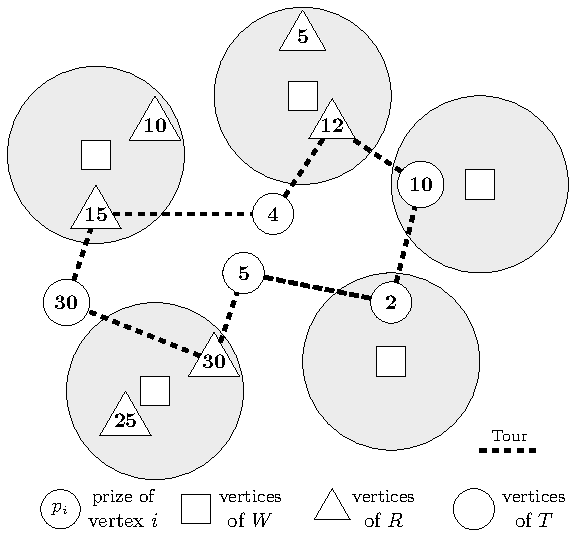
\includegraphics[width=0.45\textwidth]{pcctp-solution.pdf}
	\caption{An example of a feasible solution for a small instance with the value of $PRIZE$ set to 100.}
	\label{fig:pcctp}
\end{figure}

In their study, \citet{daSilva} present a real-world scenario for the Prize Collecting Covering Tour Problem (PCCTP). In this scenario, the vertices in set $T$ represent essential cities that need to be visited by itinerant vehicles providing social services. The vertices in set $R$, on the other hand, refer to optional stop locations for the vehicles. Set $W$ includes locations that are difficult to reach, requiring the vehicles to pass through a location within a coverage distance of $D$ to serve their residents, whether in $T$ or $R$. To ensure that the vehicle release is economically feasible, a minimum number of residents must be served, and each vertex's prize represents the population of each city. The total prize collected represents the minimum total population of residents that must be served.

Another real-life application of the PCCTP is in public transportation. For instance, a public transit system may have to plan the optimal route for a bus or train that covers a set of stations with varying demands, where each station has a certain prize representing the number of passengers to be picked up or dropped off. However, it may not be possible or cost-effective to stop at all the stations, and some stations may have to be skipped. In such a scenario, the PCCTP can be used to find the optimal route that covers the stations with the highest prizes while minimizing the cost of the route. This problem can also be extended to include additional constraints, such as time limits or the maximum number of passengers that can be carried on the vehicle.

The paper is organized as follows. Section \ref{sec:grasp} provides a brief overview of the literature on PCCTP and describes the state-of-the-art heuristic in detail. Section \ref{sec:datamining} explains the proposed data mining approaches. In Section \ref{sec:computationalresults}, we present and analyze the computational results. Finally, in Section \ref{sec:conclusions}, we draw conclusions and highlight future work.

\section{The state-of-the-art heuristic}

\label{sec:grasp}

Few authors have discussed the PCCTP before and some solution methods have been presented. \citep{lyra2004problema} introduced the PCCTP and as solution methods, proposed a mathematical formulation that makes use of flow constraints to eliminate sub-tours, and a GRASP-based heuristic  \citep{grasp03}   associated with a VNS (Variable Neighbourhood Search) metaheuristic \citep{mladenovic97}.  Also, a path-relinking strategy was used as an intensification component for trying to improve solutions.

Next, \citet{silva2009problema} introduced  six new heuristics,  which are based on the ILS (Iterated Local Search) metaheuristic and evolutionary algorithms. Finally, \citet{daSilva} proposed GRASP-based heuristic embedded with a GENIUS \citep{genius} and Random VND \citep{mladenovic12} heuristics (GRASP-GENIUS-RVND). In this heuristic, the GENIUS performed the initial solution generation, while RVND was responsible for the local search of the GRASP. As far as the authors know, the GRASP-GENIUS-RVND is the state-of-the-art heuristic for the PCCTP, in terms of quality solution and CPU time.


\subsection{GRASP-GENIUS-RVND}

The GRASP-GENIUS-RVND \citep{daSilva} is based on the GRASP (Greedy Randomised Adaptive Search Procedure) metaheuristic \citep{grasp03}. GRASP is based on a multi-start strategy, in which many initial solutions are generated through repeated applications of a semi-greedy process. At each multi-start iteration, given a constructed solution $S$, its neighbourhood $N(S)$ is explored by a local search, in order to find a better solution. The iterative process of performing the two phases, initial solution generation, and local search, is interrupted according to a stopping criterion, which can be a maximum number of interactions, a target solution value, or timeout.

\citet{daSilva} developed the solution generation phase based on the GENIUS heuristic \citep{genius} adapted for the PCCTP, while in the other phase, some moves were devised and combined in an RVND (Random Variable neighbourhood Descent) framework \citep{mladenovic97}.


\subsubsection{GENIUS}

The GENIUS heuristic \citep{genius} is implemented with  two steps: a construction approach, the GENI step (Generalized Insertion), and an improvement procedure, the Unstringing and Stringing (US) step. 

GENI is a method with a generalized insertion. Its main feature is that the evaluation of possible insertion of vertices is basically not limited to the positions between consecutive vertices.
The US step involves removing a vertex from the tour and reinserting it in another position, in each iteration, to improve the current solution. When there are no more possibilities for improvement, this process stops.


In the construction phase, we start by randomly selecting three vertices from $T$ to generate a partial tour. Then, as long as there are vertices of $T$ outside the tour, the $PRIZE$ has not been reached, and there are any uncovered vertices $w \in W $, we  perform the following steps: i) create a candidate list (CL), which contains all vertices outside the tour; ii) obtain a restricted candidate list (RCL) which is composed of the best quality vertices from CL; iii) a vertex is randomly selected from RCL and inserted in the tour by a GENIUS procedure; iv) try to improve the tour by applying the US method. The pseudo-code of the GENIUS process is given in the algorithm \ref{alg:genius_PCCTP}.


As per the findings of \citet{daSilva}, a vertex is included in the Restricted Candidate List (RCL) if its incremental cost is less than the threshold of $c^{min} + (\alpha \times (c^{max}-c^{min}))$, where $c^{min}$ and $c^{max}$ represent the minimum and maximum incremental costs in CL, respectively. Here, the parameter $\alpha \in [0,1]$ denotes the level of greediness in the heuristic. A higher value of $\alpha$ corresponds to a lesser degree of greediness.

We have used the following  greedy function (Equation \ref{custo_inc} to compute the incremental cost, which takes into account the insertion of a vertex $v$ between vertices $i$ and $j$.

\begin{flalign}
g(v) = \displaystyle \min_{i,j \in V : i \neq j} \left(c_{iv} + c_{vj}  - c_{ij}\right) \label{custo_inc}
\end{flalign}

\noindent where $c_{ij}$, $c_{iv}$ and $c_{vj}$ are the costs of the edges $(i,j)$, $(i,v)$ and $(v,j)$, respectively.

\begin{algorithm}[ht]
	%	\algsetup{linenosize=\scriptsize}
	\caption{\hspace{-1mm}: GENIUS($seed$,$\alpha$)}
	\label{alg:genius_PCCTP}
	%	{\footnotesize
		{\footnotesize
	\begin{algorithmic}[1]
		%			\REQUIRE $seed$, $\alpha$
		\STATE $i, j, k \gets \texttt{SelectRandom}(T,seed)$;
		\STATE $S \gets \cup$ $\{i, j, k\}$;
% 		\STATE $CL \gets V$;
		\STATE $CL \gets V \setminus \{i,j,k\}$
		\WHILE{$(\exists$ $t \in T$ : $t \notin S )$ \textbf{or} $(\exists$ not covered $w \in W\space)$ \textbf{or} (\textit{PRIZE} not collected) }
		\STATE $RCL \gets \texttt{setRCL}(CL, \alpha)$;
		\STATE $v \gets \texttt{SelectRandom}(RCL,seed)$;
		\STATE $GENI(S,v)$;
		\STATE $CL \gets CL \backslash {v} $;
		\ENDWHILE
		\STATE $US(S)$; \textit{//tour improvement}\\
		\RETURN $S$;
	\end{algorithmic}
		}
\end{algorithm}

\subsubsection{RVND}
Following the GRASP construction phase, the generated solution is subjected to a local search using the Random VND technique \citep{mladenovic12}. The VND is a local search metaheuristic proposed by \citet{mladenovic97} that employs several neighbourhood structures. Given an ordered list of neighbourhoods, initially, the VND explores the first neighbourhood of $S$, $N^k(S)$, and if a better solution cannot be discovered, the next $N^{(k + 1)}(S) $  neighbourhood is investigated. Otherwise, it will go back to the first neighbourhood on the list. When all neighbourhood structures have been explored, the algorithm comes to a halt and returns the best solution found. For their heuristic, \citet{daSilva} used the RVND instead of the traditional VND in which there is no neighbourhood order.

The RVND is detailed in the pseudo-code of Algorithm \ref{alg:vnd}, and it starts by shuffling the list of neighbourhood structures. Then, we can see that the counter $k$ is incremented by one to try the next neighbourhood if the current solution is not improved.
Otherwise, the current neighbourhood's local optimal solution is achieved, and $k$ is set back to 1 for restarting the loop for the newly accepted solution.
When there is no chance of improving $S$, that is, $k > k_{max}$, one returns the best current solution.

RVND is described in detail in the pseudo-code of Algorithm \ref{alg:vnd}. It first scrambles the list of neighbourhood structures. Then, we can see that if the current solution is not improved, the counter $k$ will increase by 1 to try the next neighbourhood. Otherwise, we obtain the local optimal solution of the current neighbourhood and we set $k$ to 1 to restart the loop for the newly accepted solution. When there are no neighbours to improve $S$, that is, $k> k_{max}$, the algorithm returns the current best solution.


For RVND, we have used the 15 neighbourhood structures introduced in \citet{daSilva}, which are based on TSP's classic movements \textit{swap} and \textit{shift}, as well as heuristics as GENIUS and the cheapest insert.


\begin{algorithm}
\caption{\hspace{-1mm}: RVND($S, N$)}
\label{alg:vnd}
{\footnotesize
\begin{algorithmic}[1]
\STATE Set a random order for the neighbourhood structures in $N$.
\STATE Initialise $k$ to $1$.
\WHILE{$k \leq k_{max}$}
\STATE Generate the first improving solution $S'$ in $N^{(k)}(S)$.
\IF{$S'$ is better than $S$}
\STATE Set $S$ to $S'$.
\STATE Set $k$ to $1$.
\ELSE
\STATE Increment $k$ by $1$.
\ENDIF
\ENDWHILE
\RETURN $S$.
\end{algorithmic}
}
\end{algorithm}

\section{Data mining}

\label{sec:datamining}

Data mining is the process of discovering patterns and relationships in large data sets. In a transaction database, where each transaction corresponds to a set of items in the application domain, frequent item sets can be extracted. A frequent item set is a subset of items in the domain that occurs in at least a certain minimum percentage of transactions in the database, called the support.


The frequent item-set mining (FIM) problem involves identifying all frequent item sets in the database with a minimum support value specified as an input parameter. For example, if the minimum support is set to 0.05, then a set of items is considered frequent if it appears in at least 5\% of the transactions.

Maximal frequent item sets are another type of pattern that can be mined. A maximal frequent item set is a frequent item set that is not a subset of any other frequent item set. For example, {a, b, c} is a maximal frequent item set if it is frequent and there is no other frequent item set that contains {a, b, c} as a subset.



Let us consider $E$ as a set of application elements, $t$ as a transaction that is a subset of $E$, and $D$ as a set of transactions. A set of frequent items $F$, with a support of $sup$, is a subset of $E$ that appears in at least $(sup \times 100)\%$ of transactions in $D$. Thus, the problem of identifying all sets of frequent items in $D$ with minimal support, $sup_{min}$, specified as an input parameter, is known as the frequent item-set mining (FIM) problem. Several algorithms have been proposed in the literature to solve this problem efficiently, such as Apriori \cite{agrawal1994fast} and FP-Growth \cite{han2000mining}. The FP-max* algorithm \cite{goethals04}, which is available at \url{http://fimi.uantwerpen.be/}, was introduced to efficiently mine sets of maximal frequent items \cite{grahne2003efficiently}.
	
\subsection{Hybridisation with data mining}


In its original form, GRASP lacks long-term memory since it restarts the search process in each iteration independently \cite{aloise2011adaptive}. However, some proposals in the literature suggest maintaining information from previous iterations to enhance the search process in future iterations \cite{fleurent1999improved, italo, rochat1995probabilistic, plastino2011hybrid, plastino2014adaptive, ribeiro2006hybridization}. One approach to improve GRASP is to combine it with data mining, as proposed by \citet{ribeiro2006hybridization} to solve the Set Packing Problem. This hybridisation approach has shown promising results in terms of solution quality and execution time. The idea is to extract patterns from sub-optimal solutions and use them to guide the search for better solutions efficiently.


The approach taken by \citet{ribeiro2006hybridization} to enhance the original GRASP involves dividing it into two parts. The first part generates a set of high-quality solutions (elite set), which is then subjected to data mining to extract patterns. In the second part, a pattern from the set of extracted patterns is used in each iteration to construct an initial solution using an adapted construction method. This approach has been successful in various optimisation problems, leading to its adoption in this study to solve the PCCTP.

The GRASP with data mining approach was initially applied to optimization problems that use sets of elements to represent solutions. However, this approach cannot be directly applied to problems where the order of the elements is crucial to the solution. In \citet{guerine14}, a modified GRASP with data mining was proposed for a TSP variant, where arc mining was used instead of vertex mining to preserve the order of vertices. This involved mapping each pair of vertices to a unique identifier, which was then used in the FIM technique.


In the study by \citet{guerine14}, a mapping technique for solutions was utilised. To obtain a unique identifier for a pair of sequential vertices represented by the edge $(i,j)$, the formula $a_{ij} = (i \times | V |) + j$ was employed, where $|V|$ is the total number of vertices in the problem. Once the pattern is extracted, a reverse mapping process is performed by obtaining $i = (a_{ij}$ $div$ $|V|)$ and $j = (a_{ij}$ $mod$ $|V|)$ from the identifier $a_{ij}$, where $div$ and $mod$ are mathematical operators used to obtain the quotient and remainder of the division, respectively.

As the PCCTP solutions also depend on the order of vertices, the mapping strategy used in \citet{guerine14} was adopted for this study. In the following section, we will present the hybrid heuristic that combines GRASP-GENIUS-RVND with data mining.

\subsection{DM-GRASP}

The proposed DM-GRASP in this study is based on the approach of \citet{guerine14} and is composed of two phases, each with half of the total iterations, separated by a data mining process. In the first phase, which is the same as the original GRASP-GENIUS-RVND heuristic, the best solutions found are saved in an elite set $M$ with a capacity of $cap$. A solution $S$ is considered for insertion in $M$ if it is better than the worst solution of $M$, or if $M$ is not yet full. Additionally, $M$ does not allow for identical solutions.


Following the first phase, the data mining process is executed to produce a set of patterns with minimum support of $sup_{min}$ or higher. The second phase utilises one pattern from the pattern set to create an initial solution through an adjusted constructive method in every iteration. The algorithm concludes by returning the best solution found. The DM-GRASP algorithm for the PCCTP is outlined in Algorithm \ref{alg:dm-grasp}.

In line 1, all sets and variables of the algorithm are initialised. In the first phase of the strategy (lines 2 to 10), which corresponds to the first half of the iterations, the algorithm remains the same as the original GRASP-GENIUS-RVND, except for the presence of the function \texttt{UpdateEliteSet}($M, S'', cap$) (line 8). This function inserts $S''$, which is a solution obtained by RVND, into $M$ if $S''$ is unique in $M$ and its cost is less than the worst solution in $M$. After the end of the first $k$ iterations, in line 11 the mining procedure extracts $t$ patterns from the elite set, and these patterns are inserted in descending order of size (number of edges) in the pattern set. In this work, pattern extraction is performed by the FP-max* algorithm \cite{goethals04}, which is an efficient implementation for extracting sets of maximal frequent items.


During the second phase of the algorithm (lines 12-20), the original constructive procedure (line 14) is replaced with an adapted procedure, which is described later. First, the next largest pattern is selected using a \textit{round-robin} selection from the set of patterns ($patterns_set$), and the identifiers in the patterns are mapped back to edge form as explained previously. The remaining lines of the second phase are identical to their respective parts of the original GRASP-GENIUS-RVND. Finally, the best solution $S$ is returned at the end of all iterations (line 21).




\begin{algorithm}[!h]
	\caption{\hspace{-1mm}: \textbf{DM-GRASP}($maxIt, seed, t, cap, \alpha, sup_{min}$)}
	\label{alg:dm-grasp}
	{\footnotesize
		\begin{algorithmic}[1]		
			\STATE $S\gets \emptyset$; $f(S) \gets \infty$; $M \gets \emptyset$; $k \gets 1$; 
			\WHILE{$k \leq maxIt/2$}
			\STATE $S' \gets \texttt{GENIUS} (seed, \alpha)$;  \COMMENT{Construction phase }
			\STATE $S'' \gets \texttt{RVND} (S', seed)$; \COMMENT{Local search phase}
			\IF{$f(S'') \leq f(S)$}
			\STATE $S \gets S''$;
			\ENDIF
			\STATE \texttt{UpdateEliteSet}($M, S'', cap$);
			\STATE $k \gets k +1$;
			\ENDWHILE
			\STATE	$patterns\_set \gets$ \texttt{mine}($M, cap, t, sup_{min}$)
			\WHILE{$k \leq maxIt$}
			\STATE $padrao \gets $\texttt{selectLargestNextPattern}($patterns\_set$); 
			\STATE $S' \gets$ \texttt{GENIUS\_adapted}($seed, \alpha, pattern$);
			\STATE $S'' \gets \texttt{RVND} (S', seed)$;
				\IF{$f(S'') \leq f(S)$}
			\STATE $S \gets S''$;
			\ENDIF
			\STATE $k \gets k +1$;
			\ENDWHILE
			\RETURN $S$;
		\end{algorithmic}
	}
\end{algorithm}


The approach to generate solutions using patterns in this work is based on an adapted version of the GENIUS heuristic proposed by \citet{daSilva}. Unlike the original GENIUS construction that begins from a sub-route with three random vertices, the adapted version starts from a mined pattern. The details of this construction are outlined in Algorithm \ref{alg:genius-adaptado}.

At the beginning of the algorithm, the solution $S$ is initialised with all the edges of the pattern (line 1), and the candidate list is initialised with all problem vertices that are not yet on the route (line 2). Next, a vertex is randomly chosen from the candidate list and inserted into the route using the GENI heuristic, until $S$ is complete (lines 4 to 10). Finally, the US refinement heuristic is applied to improve $S$ (line 11), which is returned in line 12.


\begin{algorithm}[!h]
	{\small
	\caption{\hspace{-1mm}:  GENIUS\_adapted($seed, \alpha, padrao$)}
	\label{alg:genius-adaptado}
	\begin{algorithmic}[1]			
		\STATE $S \gets pattern$;
		\STATE $CL \gets V \setminus S$
		\STATE \texttt{Evaluate}($CL$);
		\WHILE {$! SolutionComplete(S)$}
			\STATE $RCL \gets buildLRC(\alpha, CL)$;
			\STATE $v \gets choose\_randomly(RCL)$;
			\STATE \texttt{GENI}($S, v$);
			\STATE $CL \gets CL \setminus \{v\}$;
			\STATE \texttt{Evaluate}($CL$);
		\ENDWHILE
		\STATE \texttt{US}($S$);
		\RETURN $S$;
	\end{algorithmic}
}
\end{algorithm}



\subsection{MDM-GRASP}

The DM-GRASP algorithm mines the elite set only once, exactly after half of the iterations. However, this work proposes and investigates another approach that involves running the data mining procedure multiple times during the algorithm's execution.

Studies in the literature \cite{barbalho2013} suggest that performing data mining multiple times can gradually improve the elite set and lead to the extraction of more refined patterns. In the proposed method, the mining procedure is applied as soon as the elite set $M$ becomes stable, and again whenever $M$ changes and becomes stable again. This new method is called Multi Data-Mining GRASP (MDM-GRASP). In the context of this work, $M$ is considered stable if its set of solutions remains unchanged for a certain number of consecutive $\omega$ iterations. This means that no good quality solutions are found during these iterations that can be added to the set.

The MDM-GRASP algorithm, shown in Algorithm \ref{alg:mdm-grasp}, iterates until the maximum number of iterations, $maxIt$, is reached. If a data mining procedure has already been executed, the algorithm obtains a new solution, $S'$, through an adapted construction method, otherwise, it applies the GRASP-GENIUS-RVND construction. The local search is then performed on $S'$, resulting in a new solution, $S''$. If the cost of $S''$ is lower than the current best cost, $f^*$, then $S$ and $f^*$ are updated. If $M$ is updated with $S''$, the non-update counter, $Iter_{sa}$, is reset to zero, otherwise, it is incremented. If $M$ remains unchanged for a certain number of consecutive iterations, $\omega$, then the mining procedure is applied, and $Iter_{sa}$ is reset to zero. The best solution is returned at the end of the algorithm.




\begin{algorithm}[h]
  {\small
	\caption{\hspace{-1mm}: MDM-GRASP($maxIt, seed, t, cap, \alpha, sup_{min}, \omega$)}	
	\label{alg:mdm-grasp}
	\begin{algorithmic}[1]
		
		\STATE $S \gets \emptyset$; $f^* \gets \infty$;  $M \gets \emptyset$; $k \gets 0$; $did\_mining \gets false$; $Iter_{sa} \gets 0$;
		
%		\WHILE{$!estavel(M)$ e $k < maxIt$}
%		\STATE (Linhas 3 a 9 do Algoritmo \ref{alg:dm-grasp});
%		
%		\ENDWHILE
		
		\WHILE{$k < maxIt$}
			\IF{$did\_mining = false$}
				\STATE $S' \gets \texttt{GENIUS} (seed, \alpha)$; 
			\ELSE
				\STATE $pattern \gets $\texttt{select\_next\_largest\_pattern}($pattern\_set$); 
				\STATE $S' \gets$ \texttt{GENIUS\_adapted}($seed, \alpha, pattern$); 
			\ENDIF
			\STATE $S'' \gets \texttt{RVND} (S', seed)$; 
			\IF{$f(S'') \leq f^*$}
			\STATE $S \gets S''$; $f^* \gets f(S'')$;
			\ENDIF
			\IF {\texttt{updateEliteSet}($M, S'', cap$)}
				\STATE $Iter_{sa} \gets 0$;
			\ELSE
				\STATE $Iter_{sa} \gets Iter_{sa} + 1$;
			\ENDIF
			\IF{$Iter_{sa} = \omega$}
				\STATE $pattern\_set \gets$ \texttt{mine} ($M,cap,t, sup_{min}$);
				\STATE $Iter_{sa} \gets 0$;
				\STATE $did\_mining\gets true$;
			\ENDIF	
			\STATE $k \gets k + 1$;
		\ENDWHILE
		\RETURN {$S$};
		
	\end{algorithmic}
}
\end{algorithm}


\section{Computational experiments and results}

\label{sec:computationalresults}

This section presents the results of computational experiments conducted to compare the proposed approaches with a state-of-the-art heuristic. It should be noted that the original implementation of GRASP-GENIUS-RVND, which serves as the basis for DM-GRASP and MDM-GRASP, was provided by the authors.

To ensure a fair comparison, all heuristics were implemented in \textit{C++} and compiled with \textit{g++ 5.4.0}. The experiments were conducted on a machine with an Intel(R) Core i7-6700 CPU operating at 3.40GHz and 16GB of RAM.


\subsection{Instances}

Instances used in this work were proposed by \citet{silva2009problema} and originally used in \citet{daSilva}. The instances consist of 144 test problems obtained from the travelling salesman problem (TSP) available in the TSPLIB repository \citep{reinelt1991tsplib}. To avoid the problem of the PCCTP becoming a CTP instance, the collection of prizes associated with the vertices in $T$ alone is insufficient.

Each instance is named after its original name in the TSPLIB, with additional information about the subsets $R$, $T$, and $W$, as well as the percentage of the total $PRIZE$ that must be collected \citep{silva2009problema}. For example, the instance \textit{a280\_R56\_T168\_W56\_50} has 280 vertices in total, 56 of which are optional ($R$), 168 are mandatory ($T$), 56 must be covered ($W$), and 50\% of the total prize must be collected. These instances are publicly available in a Mendeley repository \citep{pcctspMendely}.

\subsection{DM-GRASP and MDM-GRASP results}

The DM-GRASP and MDM-GRASP algorithms used the same value for the $maxIt$ parameter as the state-of-the-art heuristic. The minimum support for both algorithms was set to 20\% as it provided a better trade-off between solution quality and computation time than the other values tested. 


Thirty-seven instances were used for the experiments, with ten runs for each support configuration and different seeds for each run. The support values were tested only from 10\% to 50\% as there were no data mining occurrences for $sup_min$= 60\% in any of the tested instances. The complete results are available in the Mendeley repository.



  After tuning the minimum support, the remaining 107 instances were used for further experiments, and the results are presented in Tables \ref{tab:dm-grasp} and \ref{tab:mdm-grasp} for DM-GRASP and MDM-GRASP, respectively. The tables show the best solution (BS), average solution (AS), and average time spent (AT) in seconds for each strategy. The best results are highlighted in bold, and columns $Dif_{as}$ and $Dif_{T}$ represent the percentage difference between the compared heuristics for the average solution obtained and CPU time spent. In Table \ref{tab:dm-grasp}, Heur1 corresponds to GRASP-GENIUS-RVND, while Heur2 represents DM-GRASP. In Table \ref{tab:mdm-grasp}, Heur1 refers to DM-GRASP, and Heur2 represents MDM-GRASP.





\begin{align}
Dif_{T} = 100 \times \frac{(T_{Heur2} - T_{Heur1})}{T_{Heur1}}
\label{eq:time}
\end{align}



% {\footnotesize
	\begin{flalign}
	Dif_{BS} = 100 \times \frac{(BS_{Heur2} - BS_{Heur1})}{BS_{Heur1}}
\label{eq:as}
	\end{flalign}
% }

{\scriptsize
	\begin{longtable}{lrrrrrrrr}
		\caption{Comparison between GRASP-GENIUS-RVND and DM-GRASP.}
		\label{tab:dm-grasp}\\
		\hline
		& \multicolumn{3}{c}{GRASP-GENIUS-RVND} & \multicolumn{5}{c}{DM-GRASP} \\
		\cline{2-9}
		%
		%
		Instance & \begin{tabular}[c]{@{}l@{}}BS \end{tabular} & \begin{tabular}[c]{@{}l@{}}AS\end{tabular} & \begin{tabular}[r]{@{}l@{}}AT \end{tabular} & \begin{tabular}[r]{@{}l@{}}BS\end{tabular} & \begin{tabular}[c]{@{}l@{}}AS\end{tabular} & \begin{tabular}[r]{@{}l@{}}AT\end{tabular} & \begin{tabular}[c]{@{}l@{}}$Dif_{BS}$\end{tabular} & \begin{tabular}[c]{@{}l@{}}$Dif_{AT}$\end{tabular} \\
		\hline
		\endhead	
		att48\_R9\_T10\_W29\_25 & \textbf{2291} & \textbf{2291.00} & 0.82 & \textbf{2291} & 2291.27 & \textbf{0.77} & -0.01 & 6.70 \\
		att48\_R9\_T29\_W10\_50 & \textbf{2824} & \textbf{2824.00} & 4.59 & \textbf{2824} & \textbf{2824.00} & \textbf{3.79} & 0.00 & 17.45 \\
		att48\_R16\_T16\_W16\_75 & \textbf{2650} & \textbf{2650.00} & 3.71 & \textbf{2650} & \textbf{2650.00} & \textbf{2.98} & 0.00 & 19.68 \\
		berlin52\_R9\_T11\_W32\_25 & \textbf{4861} & \textbf{4861.00} & 0.86 & \textbf{4861} & \textbf{4861.00} & \textbf{0.78} & 0.00 & 8.32 \\
		berlin52\_R16\_T18\_W18\_50 & \textbf{5186} & \textbf{5186.00} & 4.57 & \textbf{5186} & \textbf{5186.00} & \textbf{4.13} & 0.00 & 9.80 \\
		berlin52\_R9\_T32\_W11\_75 & \textbf{6916} & \textbf{6916.00} & 5.99 & \textbf{6916} & \textbf{6916.00} & \textbf{5.87} & 0.00 & 2.00 \\
		bier127\_R24\_T77\_W26\_25 & \textbf{98597} & 98700.70 & 79.45 & \textbf{98597} & \textbf{98648.20} & \textbf{65.52} & 0.05 & 17.52 \\
		bier127\_R24\_T26\_W77\_50 & \textbf{74745} & \textbf{74745.00} & 22.29 & \textbf{74745} & \textbf{74745.00} & \textbf{16.80} & 0.00 & 24.63 \\
		bier127\_R43\_T42\_W42\_75 & \textbf{98311} & 98390.90 & 101.08 & \textbf{98311} & \textbf{98325.40} & \textbf{88.57} & 0.07 & 12.37 \\
		brazil58\_R18\_T20\_W20\_25 & \textbf{19417} & \textbf{19417.00} & 4.02 & \textbf{19417} & \textbf{19417.00} & \textbf{3.14} & 0.00 & 22.04 \\
		brazil58\_R11\_T35\_W12\_50 & \textbf{23312} & \textbf{23312.00} & 8.12 & \textbf{23312} & \textbf{23312.00} & \textbf{5.90} & 0.00 & 27.26 \\
		brazil58\_R11\_T12\_W35\_75 & \textbf{20466} & \textbf{20466.00} & 1.75 & \textbf{20466} & \textbf{20466.00} & \textbf{1.43} & 0.00 & 18.09 \\
		brg180\_R36\_T36\_W108\_25 & \textbf{550} & \textbf{550.00} & 22.64 & \textbf{550} & \textbf{550.00} & \textbf{20.72} & 0.00 & 8.52 \\
		brg180\_R60\_T60\_W60\_50 & \textbf{2360} & \textbf{2360.00} & \textbf{134.29} & \textbf{2360} & \textbf{2360.00} & 135.35 & 0.00 & -0.79 \\
		brg180\_R36\_T108\_W36\_75 & \textbf{2210} & \textbf{2211.00} & 185.08 & \textbf{2210} & 2215.00 & \textbf{180.94} & -0.18 & 2.23 \\
		ch130\_R44\_T43\_W43\_25 & \textbf{4383} & \textbf{4383.00} & 21.78 & \textbf{4383} & 4383.90 & \textbf{18.96} & -0.02 & 12.95 \\
		ch130\_R26\_T26\_W78\_50 & \textbf{4139} & \textbf{4139.00} & 16.65 & \textbf{4139} & \textbf{4139.00} & \textbf{12.46} & 0.00 & 25.21 \\
		ch130\_R26\_T78\_W26\_75 & \textbf{5287} & \textbf{5303.80} & 87.47 & 5304 & 5306.50 & \textbf{72.20} & -0.05 & 17.46 \\
		ch150\_R50\_T50\_W50\_25 & \textbf{4778} & 4800.20 & 58.63 & \textbf{4778} & \textbf{4797.80} & \textbf{42.89} & 0.05 & 26.85 \\
		ch150\_R30\_T90\_W30\_50 & \textbf{5239} & \textbf{5245.50} & 131.38 & \textbf{5239} & 5247.80 & \textbf{103.98} & -0.04 & 20.85 \\
		ch150\_R30\_T30\_W90\_75 & \textbf{4292} & \textbf{4292.00} & 20.33 & \textbf{4292} & \textbf{4292.00} & \textbf{16.51} & 0.00 & 18.77 \\
		d198\_R39\_T40\_W119\_25 & \textbf{10916} & \textbf{10916.00} & 53.19 & \textbf{10916} & \textbf{10916.00} & \textbf{38.57} & 0.00 & 27.49 \\
		d198\_R39\_T119\_W40\_50 & \textbf{13598} & 13602.60 & 448.89 & \textbf{13598} & \textbf{13599.90} & \textbf{367.46} & 0.02 & 18.14 \\
		d198\_R66\_T66\_W66\_75 & \textbf{12907} & \textbf{12924.40} & 534.73 & \textbf{12907} & 12927.90 & \textbf{424.74} & -0.03 & 20.57 \\
		eil51\_R17\_T17\_W17\_25 & \textbf{273} & \textbf{273.00} & 2.51 & \textbf{273} & \textbf{273.00} & \textbf{2.32} & 0.00 & 7.51 \\
		eil51\_R9\_T11\_W31\_50 & \textbf{248} & \textbf{248.00} & 1.03 & \textbf{248} & \textbf{248.00} & \textbf{0.85} & 0.00 & 17.37 \\
		eil51\_R9\_T31\_W11\_75 & \textbf{348} & 348.50 & 5.18 & \textbf{348} & \textbf{348.10} & \textbf{4.96} & 0.11 & 4.30 \\
		eil76\_R14\_T46\_W16\_25 & \textbf{387} & \textbf{387.00} & 12.18 & \textbf{387} & \textbf{387.00} & \textbf{10.26} & 0.00 & 15.76 \\
		eil76\_R24\_T26\_W26\_50 & \textbf{338} & \textbf{338.00} & 10.54 & \textbf{338} & \textbf{338.00} & \textbf{8.20} & 0.00 & 22.21 \\
		eil76\_R14\_T16\_W46\_75 & \textbf{332} & \textbf{332.00} & 2.92 & \textbf{332} & \textbf{332.00} & \textbf{2.58} & 0.00 & 11.47 \\
		eil101\_R19\_T21\_W61\_25 & \textbf{356} & \textbf{356.00} & 7.73 & \textbf{356} & \textbf{356.00} & \textbf{5.99} & 0.00 & 22.53 \\
		eil101\_R19\_T61\_W21\_50 & \textbf{506} & \textbf{506.00} & 38.8 & \textbf{506} & \textbf{506.00} & \textbf{32.53} & 0.00 & 16.15 \\
		eil101\_R33\_T34\_W34\_75 & \textbf{462} & 463.40 & 40.06 & \textbf{462} & \textbf{463.10} & \textbf{37.64} & 0.06 & 6.03 \\
		gr48\_R16\_T16\_W16\_25 & \textbf{3571} & \textbf{3571.00} & 1.82 & \textbf{3571} & \textbf{3571.00} & \textbf{1.39} & 0.00 & 23.95 \\
		gr48\_R9\_T10\_W29\_50 & \textbf{3524} & \textbf{3524.00} & 0.79 & \textbf{3524} & \textbf{3524.00} & \textbf{0.77} & 0.00 & 2.00 \\
		gr48\_R9\_T29\_W10\_75 & \textbf{4415} & \textbf{4415.00} & 4.16 & \textbf{4415} & \textbf{4415.00} & \textbf{3.91} & 0.00 & 5.96 \\
		gr96\_R18\_T58\_W20\_25 & \textbf{42746} & 42749.60 & 30.44 & \textbf{42746} & \textbf{42746.00} & \textbf{25.15} & 0.01 & 17.40 \\
		gr96\_R32\_T32\_W32\_50 & \textbf{35461} & \textbf{35461.00} & 58.09 & \textbf{35461} & \textbf{35461.00} & \textbf{47.67} & 0.00 & 17.95 \\
		gr96\_R18\_T20\_W58\_75 & \textbf{30015} & \textbf{30015.00} & 9.67 & \textbf{30015} & \textbf{30015.00} & \textbf{7.30} & 0.00 & 24.50 \\
		gr120\_R40\_T40\_W40\_25 & \textbf{4301} & \textbf{4301.00} & 27.8 & \textbf{4301} & \textbf{4301.00} & \textbf{19.35} & 0.00 & 30.40 \\
		gr120\_R24\_T72\_W24\_50 & \textbf{5159} & 5163.70 & 60.02 & \textbf{5159} & \textbf{5161.80} & \textbf{49.16} & 0.04 & 18.10 \\
		gr120\_R24\_T24\_W72\_75 & \textbf{4275} & \textbf{4275.00} & 13.73 & \textbf{4275} & \textbf{4275.00} & \textbf{10.25} & 0.00 & 25.38 \\
		gr137\_R26\_T28\_W83\_25 & \textbf{39305} & \textbf{39305.00} & 15.82 & \textbf{39305} & \textbf{39305.00} & \textbf{13.66} & 0.00 & 13.62 \\
		gr137\_R45\_T46\_W46\_50 & \textbf{46122} & \textbf{46122.00} & 180.51 & \textbf{46122} & \textbf{46122.00} & \textbf{137.59} & 0.00 & 23.78 \\
		gr137\_R26\_T83\_W28\_75 & \textbf{58720} & 58778.00 & 116.18 & \textbf{58720} & \textbf{58748.20} & \textbf{90.59} & 0.05 & 22.02 \\
		hk48\_R9\_T29\_W10\_25 & \textbf{9708} & 9708.60 & 3.82 & \textbf{9708} & \textbf{9708.00} & \textbf{3.50} & 0.01 & 8.24 \\
		hk48\_R16\_T16\_W16\_50 & \textbf{7593} & \textbf{7593.00} & 2.11 & \textbf{7593} & \textbf{7593.00} & \textbf{1.99} & 0.00 & 5.82 \\
		hk48\_R9\_T10\_W29\_75 & \textbf{7803} & \textbf{7803.00} & 0.94 & \textbf{7803} & \textbf{7803.00} & \textbf{0.87} & 0.00 & 7.95 \\
		kroA100\_R20\_T20\_W60\_25 & \textbf{10848} & \textbf{10848.00} & 5.39 & \textbf{10848} & \textbf{10848.00} & \textbf{4.67} & 0.00 & 13.29 \\
		kroA100\_R20\_T60\_W20\_50 & \textbf{16544} & \textbf{16544.00} & 34.1 & \textbf{16544} & \textbf{16544.00} & \textbf{28.29} & 0.00 & 17.03 \\
		kroA100\_R34\_T33\_W33\_75 & \textbf{14606} & \textbf{14606.00} & 43.86 & \textbf{14606} & \textbf{14606.00} & \textbf{33.70} & 0.00 & 23.15 \\
		kroA150\_R50\_T50\_W50\_25 & \textbf{14382} & 14453.20 & 115.63 & 14410 & \textbf{14453.10} & \textbf{104.29} & 0.00 & 9.81 \\
		kroA150\_R30\_T30\_W90\_50 & \textbf{12846} & 12964.60 & 41.69 & 12882 & \textbf{12915.00} & \textbf{36.51} & 0.38 & 12.43 \\
		kroA150\_R30\_T90\_W30\_75 & \textbf{21974} & 21991.00 & 166.24 & \textbf{21974} & \textbf{21987.00} & \textbf{130.56} & 0.02 & 21.47 \\
		kroA200\_R40\_T120\_W40\_25 & \textbf{23495} & \textbf{23495.80} & 303.96 & \textbf{23495} & 23497.80 & \textbf{246.14} & -0.01 & 19.02 \\
		kroA200\_R68\_T66\_W66\_50 & \textbf{17297} & 17323.90 & 727.36 & \textbf{17297} & \textbf{17321.70} & \textbf{530.35} & 0.01 & 27.09 \\
		kroA200\_R40\_T40\_W120\_75 & \textbf{15197} & \textbf{15197.00} & 93.34 & \textbf{15197} & \textbf{15197.00} & \textbf{80.03} & 0.00 & 14.26 \\
		kroB100\_R20\_T60\_W20\_25 & \textbf{18406} & \textbf{18406.00} & 29.93 & \textbf{18406} & \textbf{18406.00} & \textbf{25.11} & 0.00 & 16.09 \\
		kroB100\_R34\_T33\_W33\_50 & \textbf{14160} & \textbf{14164.00} & 55.5 & \textbf{14160} & \textbf{14164.00} & \textbf{43.23} & 0.00 & 22.10 \\
		kroB100\_R34\_T33\_W33\_75 & \textbf{14768} & \textbf{14768.00} & 52.13 & \textbf{14768} & \textbf{14768.00} & \textbf{37.30} & 0.00 & 28.44 \\
		kroB150\_R30\_T30\_W90\_25 & \textbf{11467} & \textbf{11477.80} & 23.54 & \textbf{11467} & \textbf{11477.80} & \textbf{20.07} & 0.00 & 14.74 \\
		kroB150\_R50\_T50\_W50\_50 & \textbf{15388} & \textbf{15414.80} & 181.73 & \textbf{15388} & 15418.20 & \textbf{137.35} & -0.02 & 24.42 \\
		kroB150\_R30\_T90\_W30\_75 & \textbf{21489} & \textbf{21541.70} & 138.07 & \textbf{21489} & 21557.50 & \textbf{114.85} & -0.07 & 16.82 \\
		kroB200\_R40\_T120\_W40\_25 & 24030 & 24057.80 & 320.21 & \textbf{23954} & \textbf{24026.50} & \textbf{257.15} & 0.13 & 19.69 \\
		kroB200\_R40\_T40\_W120\_50 & \textbf{14103} & \textbf{14126.60} & 145.33 & 14125 & 14134.20 & \textbf{113.80} & -0.05 & 21.69 \\
		kroB200\_R68\_T66\_W66\_75 & \textbf{19459} & 19493.10 & 614.45 & \textbf{19459} & \textbf{19472.40} & \textbf{469.76} & 0.11 & 23.55 \\
		kroC100\_R20\_T60\_W20\_25 & \textbf{16785} & \textbf{16785.00} & 31.5 & \textbf{16785} & \textbf{16785.00} & \textbf{24.50} & 0.00 & 22.21 \\
		kroC100\_R34\_T33\_W33\_50 & \textbf{13235} & \textbf{13235.00} & 50.06 & \textbf{13235} & \textbf{13235.00} & \textbf{39.18} & 0.00 & 21.73 \\
		kroC100\_R20\_T20\_W60\_75 & \textbf{12582} & \textbf{12582.00} & 11.39 & \textbf{12582} & \textbf{12582.00} & \textbf{7.84} & 0.00 & 31.13 \\
		kroE100\_R20\_T60\_W20\_25 & \textbf{17199} & 17206.50 & 27.83 & \textbf{17199} & \textbf{17199.00} & \textbf{22.99} & 0.04 & 17.40 \\
		kroE100\_R20\_T20\_W60\_50 & \textbf{10586} & \textbf{10586.00} & 10.97 & \textbf{10586} & \textbf{10586.00} & \textbf{7.93} & 0.00 & 27.70 \\
		kroE100\_R34\_T33\_W33\_75 & \textbf{14622} & \textbf{14622.00} & 47.92 & \textbf{14622} & \textbf{14622.00} & \textbf{36.03} & 0.00 & 24.81 \\
		lin105\_R21\_T21\_W63\_25 & \textbf{8893} & \textbf{8893.00} & 7.72 & \textbf{8893} & \textbf{8893.00} & \textbf{5.97} & 0.00 & 22.61 \\
		lin105\_R21\_T63\_W21\_50 & \textbf{11583} & \textbf{11583.00} & 102.19 & \textbf{11583} & \textbf{11583.00} & \textbf{76.52} & 0.00 & 25.12 \\
		lin105\_R35\_T35\_W35\_75 & \textbf{10566} & 10566.20 & 69.05 & \textbf{10566} & \textbf{10566.00} & \textbf{54.54} & 0.00 & 21.01 \\
		pr76\_R14\_T16\_W46\_25 & \textbf{66007} & \textbf{66007.00} & 2.55 & \textbf{66007} & \textbf{66007.00} & \textbf{2.21} & 0.00 & 13.37 \\
		pr76\_R24\_T26\_W26\_50 & \textbf{74539} & 74540.50 & 15.99 & \textbf{74539} & \textbf{74540.00} & \textbf{14.34} & 0.00 & 10.31 \\
		pr76\_R14\_T46\_W16\_75 & \textbf{90862} & \textbf{90862.00} & 16.04 & \textbf{90862} & \textbf{90862.00} & \textbf{13.66} & 0.00 & 14.84 \\
		pr107\_R20\_T65\_W22\_25 & \textbf{40994} & \textbf{40994.00} & 33.53 & \textbf{40994} & \textbf{40994.00} & \textbf{24.82} & 0.00 & 25.99 \\
		pr107\_R20\_T22\_W65\_50 & \textbf{35869} & \textbf{35869.00} & 4.8 & \textbf{35869} & \textbf{35869.00} & \textbf{3.93} & 0.00 & 18.14 \\
		pr107\_R35\_T36\_W36\_75 & \textbf{37292} & 37322.00 & 36.78 & \textbf{37292} & \textbf{37309.20} & \textbf{26.83} & 0.03 & 27.05 \\
		pr124\_R42\_T41\_W41\_25 & \textbf{35465} & \textbf{35465.00} & 61.79 & \textbf{35465} & \textbf{35465.00} & \textbf{51.94} & 0.00 & 15.94 \\
		pr124\_R24\_T75\_W25\_50 & \textbf{49160} & \textbf{49160.00} & 115.84 & \textbf{49160} & 49164.40 & \textbf{87.77} & -0.01 & 24.23 \\
		pr124\_R24\_T25\_W75\_75 & \textbf{34359} & \textbf{34359.00} & 21.25 & \textbf{34359} & \textbf{34359.00} & \textbf{14.65} & 0.00 & 31.08 \\
		pr136\_R26\_T28\_W82\_25 & \textbf{47620} & \textbf{47620.00} & 11.09 & \textbf{47620} & \textbf{47620.00} & \textbf{7.77} & 0.00 & 29.95 \\
		pr136\_R46\_T45\_W45\_50 & \textbf{59445} & 59512.80 & 125.37 & \textbf{59445} & \textbf{59477.10} & \textbf{90.14} & 0.06 & 28.10 \\
		pr136\_R26\_T82\_W28\_75 & \textbf{78624} & \textbf{78629.80} & 113.31 & \textbf{78624} & 78653.60 & \textbf{82.56} & -0.03 & 27.14 \\
		pr144\_R28\_T87\_W29\_25 & \textbf{46940} & \textbf{46940.00} & 89.39 & \textbf{46940} & 46944.80 & \textbf{64.67} & -0.01 & 27.65 \\
		pr144\_R28\_T29\_W87\_50 & \textbf{30294} & \textbf{30294.00} & 18.9 & \textbf{30294} & \textbf{30294.00} & \textbf{14.97} & 0.00 & 20.79 \\
		pr144\_R48\_T48\_W48\_75 & \textbf{43713} & \textbf{43726.50} & 155.46 & \textbf{43713} & 43743.20 & \textbf{125.64} & -0.04 & 19.19 \\
		pr152\_R50\_T51\_W51\_25 & \textbf{50667} & \textbf{50667.20} & 80.99 & \textbf{50667} & 50667.30 & \textbf{61.45} & 0.00 & 24.13 \\
		pr152\_R29\_T92\_W31\_50 & \textbf{61068} & \textbf{61068.00} & 291.48 & \textbf{61068} & \textbf{61068.00} & \textbf{216.31} & 0.00 & 25.79 \\
		pr152\_R29\_T31\_W92\_75 & \textbf{49110} & \textbf{49110.00} & 49.12 & \textbf{49110} & \textbf{49110.00} & \textbf{31.83} & 0.00 & 35.19 \\
		rat99\_R19\_T20\_W60\_25 & \textbf{792} & \textbf{792.00} & 6.35 & \textbf{792} & \textbf{792.00} & \textbf{5.41} & 0.00 & 14.89 \\
		rat99\_R33\_T33\_W33\_50 & \textbf{847} & \textbf{847.00} & 24.65 & \textbf{847} & \textbf{847.00} & \textbf{20.24} & 0.00 & 17.88 \\
		rat99\_R19\_T60\_W20\_75 & \textbf{1017} & \textbf{1017.00} & 38.08 & \textbf{1017} & \textbf{1017.00} & \textbf{30.74} & 0.00 & 19.27 \\
		rat195\_R65\_T65\_W65\_25 & \textbf{1605} & 1609.10 & 344.38 & \textbf{1605} & \textbf{1606.80} & \textbf{249.12} & 0.14 & 27.66 \\
		rat195\_R39\_T39\_W117\_50 & \textbf{1199} & \textbf{1199.00} & 79.22 & \textbf{1199} & \textbf{1199.00} & \textbf{54.56} & 0.00 & 31.13 \\
		rat195\_R39\_T117\_W39\_75 & 1929 & 1938.00 & 378.31 & \textbf{1928} & \textbf{1933.80} & \textbf{286.81} & 0.22 & 24.19 \\
		rd100\_R34\_T33\_W33\_25 & \textbf{5552} & \textbf{5552.00} & 16.36 & \textbf{5552} & \textbf{5552.00} & \textbf{11.84} & 0.00 & 27.59 \\
		rd100\_R20\_T60\_W20\_50 & \textbf{6619} & 6644.80 & 32.46 & \textbf{6619} & \textbf{6635.90} & \textbf{26.44} & 0.13 & 18.54 \\
		rd100\_R20\_T20\_W60\_75 & \textbf{5421} & \textbf{5421.00} & 6.21 & \textbf{5421} & \textbf{5421.00} & \textbf{5.37} & 0.00 & 13.54 \\
		si175\_R35\_T35\_W105\_25 & \textbf{4845} & 4850.20 & 71.29 & \textbf{4845} & \textbf{4847.60} & \textbf{65.79} & 0.05 & 7.71 \\
		si175\_R35\_T105\_W35\_50 & \textbf{7011} & 7039.00 & 404.75 & \textbf{7011} & \textbf{7032.40} & \textbf{388.96} & 0.09 & 3.90 \\
		si175\_R59\_T58\_W58\_75 & 8430 & 8447.70 & 379.09 & \textbf{8428} & \textbf{8443.10} & \textbf{375.49} & 0.05 & 0.95 \\
		st70\_R14\_T14\_W42\_25 & \textbf{419} & \textbf{419.00} & 2.27 & \textbf{419} & \textbf{419.00} & \textbf{1.75} & 0.00 & 22.71 \\
		st70\_R14\_T42\_W14\_50 & \textbf{554} & \textbf{554.00} & 13.92 & \textbf{554} & \textbf{554.00} & \textbf{11.34} & 0.00 & 18.52 \\
		st70\_R22\_T24\_W24\_75 & \textbf{505} & \textbf{505.00} & 9.39 & \textbf{505} & \textbf{505.00} & \textbf{8.44} & 0.00 & 10.13 \\
		u159\_R31\_T96\_W32\_25 & \textbf{35442} & \textbf{35442.00} & 86.73 & \textbf{35442} & \textbf{35442.00} & \textbf{66.29} & 0.00 & 23.57 \\
		u159\_R31\_T32\_W96\_50 & \textbf{28613} & \textbf{28613.00} & 27.23 & \textbf{28613} & \textbf{28613.00} & \textbf{19.05} & 0.00 & 30.06 \\
		u159\_R53\_T53\_W53\_75 & \textbf{33015} & \textbf{33072.00} & 132.21 & \textbf{33015} & \textbf{33072.00} & \textbf{106.33} & 0.00 & 19.57 \\
		a280\_R94\_T93\_W93\_25 & \textbf{1717} & 1724.60 & 747.75 & 1718 & \textbf{1722.50} & \textbf{644.92} & 0.12 & 13.75 \\
		a280\_R56\_T168\_W56\_50 & \textbf{1996} & \textbf{2001.10} & 1208.35 & 1998 & \textbf{2001.10} & \textbf{1024.14} & 0.00 & 15.24 \\
		a280\_R56\_T56\_W168\_75 & \textbf{1647} & \textbf{1652.00} & 209.48 & \textbf{1647} & \textbf{1652.00} & \textbf{109.35} & 0.00 & 47.80 \\
		gil262\_R51\_T53\_W158\_25 & \textbf{1465} & 1471.30 & 226.15 & \textbf{1465} & \textbf{1468.20} & \textbf{153.66} & 0.21 & 32.05 \\
		gil262\_R88\_T87\_W87\_50 & \textbf{1678} & 1683.10 & 522.83 & \textbf{1678} & \textbf{1682.10} & \textbf{460.43} & 0.06 & 11.94 \\
		gil262\_R51\_T158\_W53\_75 & \textbf{1988} & \textbf{1996.90} & 1383.03 & 1989 & 1999.50 & \textbf{1300.50} & -0.13 & 5.97 \\
		gr202\_R39\_T122\_W41\_25 & \textbf{32162} & 32185.40 & 404.52 & \textbf{32162} & \textbf{32185.20} & \textbf{293.56} & 0.00 & 27.43 \\
		gr202\_R68\_T67\_W67\_50 & \textbf{28706} & 28747.00 & 886.79 & 28723 & \textbf{28741.70} & \textbf{719.21} & 0.02 & 18.90 \\
		gr202\_R39\_T41\_W122\_75 & \textbf{25905} & \textbf{25905.00} & 147.29 & \textbf{25905} & \textbf{25905.00} & \textbf{118.46} & 0.00 & 19.58 \\
		gr229\_R45\_T46\_W138\_25 & \textbf{61278} & 61307.30 & 79.33 & \textbf{61278} & \textbf{61280.50} & \textbf{66.34} & 0.04 & 16.37 \\
		gr229\_R45\_T138\_W46\_50 & \textbf{96707} & 97145.60 & 746.14 & \textbf{96707} & \textbf{97024.60} & \textbf{672.38} & 0.12 & 9.88 \\
		gr229\_R77\_T76\_W76\_75 & \textbf{90701} & 90838.20 & 871.34 & 90712 & \textbf{90736.30} & \textbf{702.71} & 0.11 & 19.35 \\
		lin318\_R63\_T64\_W191\_25 & \textbf{16297} & \textbf{16297.00} & 438.01 & \textbf{16297} & \textbf{16297.00} & \textbf{333.22} & 0.00 & 23.93 \\
		lin318\_R108\_T105\_W105\_50 & 23215 & 23303.00 & 4425.67 & \textbf{23137} & \textbf{23259.20} & \textbf{3973.73} & 0.19 & 10.21 \\
		lin318\_R63\_T191\_W64\_75 & 32879 & 32920.90 & 2550.26 & \textbf{32838} & \textbf{32901.90} & \textbf{2126.96} & 0.06 & 16.60 \\
		pr226\_R76\_T75\_W75\_25 & \textbf{55812} & \textbf{56455.60} & 474.67 & 56052 & 57259.20 & \textbf{311.15} & -1.42 & 34.45 \\
		pr226\_R44\_T136\_W46\_50 & \textbf{67323} & \textbf{67773.80} & 523.85 & \textbf{67323} & 67794.40 & \textbf{520.75} & -0.03 & 0.59 \\
		pr226\_R44\_T46\_W136\_75 & 50768 & 50856.00 & 753.95 & \textbf{50701} & \textbf{50768.80} & \textbf{85.75} & 0.17 & 88.63 \\
		pr264\_R52\_T53\_W159\_25 & \textbf{27693} & \textbf{27693.00} & 138.98 & \textbf{27693} & \textbf{27693.00} & \textbf{99.12} & 0.00 & 28.68 \\
		pr264\_R88\_T88\_W88\_50 & 34057 & 34120.90 & 1597.63 & \textbf{34052} & \textbf{34076.00} & \textbf{1255.50} & 0.13 & 21.41 \\
		pr264\_R52\_T159\_W53\_75 & 45157 & 45398.40 & 1116.7 & \textbf{45088} & \textbf{45276.40} & \textbf{916.70} & 0.27 & 17.91 \\
		pr299\_R59\_T180\_W60\_25 & \textbf{34671} & 34734.60 & 1518.55 & \textbf{34671} & \textbf{34701.70} & \textbf{1173.45} & 0.09 & 22.73 \\
		pr299\_R59\_T60\_W180\_50 & 20186 & \textbf{20195.70} & 403.78 & \textbf{20184} & 20215.40 & \textbf{324.81} & -0.10 & 19.56 \\
		pr299\_R101\_T99\_W99\_75 & \textbf{29711} & \textbf{29855.80} & 3219.02 & \textbf{29711} & 29872.30 & \textbf{2654.89} & -0.06 & 17.52 \\
		rd400\_R80\_T240\_W80\_25 & 10557 & 10606.90 & 5892.05 & \textbf{10543} & \textbf{10580.70} & \textbf{4969.05} & 0.25 & 15.67 \\
		rd400\_R80\_T80\_W240\_50 & \textbf{5747} & \textbf{5747.00} & 2077.88 & \textbf{5747} & \textbf{5747.00} & \textbf{1399.54} & 0.00 & 32.65 \\
		rd400\_R136\_T132\_W132\_75 & 8900 & 8929.70 & 8816.49 & \textbf{8892} & \textbf{8918.10} & \textbf{8074.28} & 0.13 & 8.42 \\
		ts225\_R45\_T45\_W135\_25 & \textbf{87889} & \textbf{88052.10} & 48.37 & \textbf{87889} & 88270.70 & \textbf{42.11} & -0.25 & 12.94 \\
		ts225\_R45\_T135\_W45\_50 & \textbf{108805} & \textbf{109113.00} & 229.37 & \textbf{108805} & 109117.00 & \textbf{225.41} & 0.00 & 1.73 \\
		ts225\_R75\_T75\_W75\_75 & 97236 & 97380.40 & 463.44 & \textbf{96959} & \textbf{97181.90} & \textbf{392.21} & 0.20 & 15.37 \\
		tsp225\_R75\_T75\_W75\_25 & \textbf{2676} & 2676.90 & 251.12 & \textbf{2676} & \textbf{2676.80} & \textbf{169.60} & 0.00 & 32.46 \\
		tsp225\_R75\_T75\_W75\_50 & \textbf{2733} & 2740.70 & 411.56 & \textbf{2733} & \textbf{2737.00} & \textbf{366.19} & 0.14 & 11.02 \\
		tsp225\_R45\_T45\_W135\_75 & \textbf{2447} & 2447.50 & 103.88 & \textbf{2447} & \textbf{2447.00} & \textbf{81.79} & 0.02 & 21.27 \\
		\hline 
 Averages &  &  &  &  &  &  & 0.011 & 19.139 \\
		\hline \\
	\end{longtable}
	
}

Based on Table \ref{tab:dm-grasp}, it can be observed that DM-GRASP outperforms GRASP-GENIUS-RVND in terms of the quality of the best solution in 11 instances, ties in 87 instances, and loses in 8 cases. For the average solution, the proposed hybrid method wins in 37 instances, ties in 52 instances, and loses in 18 instances. As reported in the literature, one of the main advantages of the data mining application is the reduction in processing time. DM-GRASP outperforms GRASP-GENIUS-RVND in terms of the average time spent in 106 instances and loses only in one instance, resulting in an average reduction of 19.28\% per instance.

\begin{scriptsize}
	\begin{longtable}{lrrrrrrrr}
		\caption{Comparison between DM-GRASP and MDM-GRASP.}
		\label{tab:mdm-grasp}\\
		\hline
		& \multicolumn{3}{c}{DM-GRASP} & \multicolumn{3}{c}{MDM-GRASP} \\
		\cline{2-9}
		%
		%
		Instance & \begin{tabular}[c]{@{}l@{}}BS\end{tabular} & \begin{tabular}[c]{@{}l@{}}AS\end{tabular} & \begin{tabular}[r]{@{}l@{}}AT\end{tabular} & \begin{tabular}[r]{@{}l@{}}BS\end{tabular} & \begin{tabular}[c]{@{}l@{}}AS\end{tabular} & \begin{tabular}[r]{@{}l@{}}AT\end{tabular} & \begin{tabular}[c]{@{}l@{}}$Dif_{ms}$\end{tabular} & \begin{tabular}[c]{@{}l@{}}$Dif_{T}$\end{tabular} \\
		\hline
		\endhead
		att48\_R9\_T10\_W29\_25 & \textbf{2291} & \textbf{2291.27} & 0.77 & \textbf{2291} & 2291.50 & \textbf{0.71} & -0.01 & 7.37 \\
		att48\_R9\_T29\_W10\_50 & \textbf{2824} & \textbf{2824.00} & 3.79 & \textbf{2824} & \textbf{2824.00} & \textbf{3.67} & 0.00 & 3.02 \\
		att48\_R16\_T16\_W16\_75 & \textbf{2650} & \textbf{2650.00} & \textbf{2.98} & \textbf{2650} & \textbf{2650.00} & 3.03 & 0.00 & -1.70 \\
		berlin52\_R9\_T11\_W32\_25 & \textbf{4861} & \textbf{4861.00} & 0.78 & \textbf{4861} & \textbf{4861.00} & \textbf{0.71} & 0.00 & 9.30 \\
		berlin52\_R16\_T18\_W18\_50 & \textbf{5186} & \textbf{5186.00} & 4.13 & \textbf{5186} & \textbf{5186.00} & \textbf{4.06} & 0.00 & 1.55 \\
		berlin52\_R9\_T32\_W11\_75 & \textbf{6916} & \textbf{6916.00} & \textbf{5.87} & \textbf{6916} & 6916.50 & 5.89 & -0.01 & -0.22 \\
		bier127\_R24\_T77\_W26\_25 & 98597 & 98648.20 & 65.52 & \textbf{98453} & \textbf{98600.10} & \textbf{64.16} & 0.05 & 2.08 \\
		bier127\_R24\_T26\_W77\_50 & \textbf{74745} & \textbf{74745.00} & 16.80 & \textbf{74745} & \textbf{74745.00} & \textbf{15.13} & 0.00 & 9.95 \\
		bier127\_R43\_T42\_W42\_75 & \textbf{98311} & \textbf{98325.40} & 88.57 & \textbf{98311} & \textbf{98325.40} & \textbf{86.69} & 0.00 & 2.13 \\
		brazil58\_R18\_T20\_W20\_25 & \textbf{19417} & \textbf{19417.00} & 3.14 & \textbf{19417} & \textbf{19417.00} & \textbf{2.96} & 0.00 & 5.57 \\
		brazil58\_R11\_T35\_W12\_50 & \textbf{23312} & \textbf{23312.00} & 5.90 & \textbf{23312} & \textbf{23312.00} & \textbf{5.66} & 0.00 & 4.17 \\
		brazil58\_R11\_T12\_W35\_75 & \textbf{20466} & \textbf{20466.00} & \textbf{1.43} & \textbf{20466} & \textbf{20466.00} & \textbf{1.43} & 0.00 & 0.36 \\
		brg180\_R36\_T36\_W108\_25 & \textbf{550} & \textbf{550.00} & \textbf{20.72} & \textbf{550} & \textbf{550.00} & 21.32 & 0.00 & -2.90 \\
		brg180\_R60\_T60\_W60\_50 & \textbf{2360} & \textbf{2360.00} & \textbf{135.35} & \textbf{2360} & \textbf{2360.00} & 137.77 & 0.00 & -1.79 \\
		brg180\_R36\_T108\_W36\_75 & \textbf{2210} & 2215.00 & \textbf{180.94} & \textbf{2210} & \textbf{2212.00} & 181.62 & 0.14 & -0.38 \\
		ch130\_R44\_T43\_W43\_25 & \textbf{4383} & \textbf{4383.90} & 18.96 & \textbf{4383} & 4384.80 & \textbf{18.27} & -0.02 & 3.66 \\
		ch130\_R26\_T26\_W78\_50 & \textbf{4139} & \textbf{4139.00} & 12.46 & \textbf{4139} & \textbf{4139.00} & \textbf{11.21} & 0.00 & 9.97 \\
		ch130\_R26\_T78\_W26\_75 & \textbf{5304} & \textbf{5306.50} & 72.20 & \textbf{5304} & \textbf{5306.50} & \textbf{71.95} & 0.00 & 0.35 \\
		ch150\_R50\_T50\_W50\_25 & \textbf{4778} & \textbf{4797.80} & 42.89 & \textbf{4778} & 4800.30 & \textbf{37.26} & -0.05 & 13.12 \\
		ch150\_R30\_T90\_W30\_50 & \textbf{5239} & 5247.80 & 103.98 & \textbf{5239} & \textbf{5247.10} & \textbf{98.91} & 0.01 & 4.88 \\
		ch150\_R30\_T30\_W90\_75 & \textbf{4292} & \textbf{4292.00} & 16.51 & \textbf{4292} & \textbf{4292.00} & \textbf{15.91} & 0.00 & 3.62 \\
		d198\_R39\_T40\_W119\_25 & \textbf{10916} & \textbf{10916.00} & 38.57 & \textbf{10916} & \textbf{10916.00} & \textbf{36.91} & 0.00 & 4.30 \\
		d198\_R39\_T119\_W40\_50 & \textbf{13598} & \textbf{13599.90} & 367.46 & \textbf{13598} & 13600.00 & \textbf{349.83} & 0.00 & 4.80 \\
		d198\_R66\_T66\_W66\_75 & \textbf{12907} & 12927.90 & 424.74 & \textbf{12907} & \textbf{12926.50} & \textbf{389.28} & 0.01 & 8.35 \\
		eil51\_R17\_T17\_W17\_25 & \textbf{273} & \textbf{273.00} & 2.32 & \textbf{273} & \textbf{273.00} & \textbf{2.30} & 0.00 & 0.84 \\
		eil51\_R9\_T11\_W31\_50 & \textbf{248} & \textbf{248.00} & \textbf{0.85} & \textbf{248} & \textbf{248.00} & 0.97 & 0.00 & -14.11 \\
		eil51\_R9\_T31\_W11\_75 & \textbf{348} & \textbf{348.10} & \textbf{4.96} & \textbf{348} & 348.40 & 4.98 & -0.09 & -0.39 \\
		eil76\_R14\_T46\_W16\_25 & \textbf{387} & \textbf{387.00} & 10.26 & \textbf{387} & \textbf{387.00} & \textbf{9.65} & 0.00 & 5.94 \\
		eil76\_R24\_T26\_W26\_50 & \textbf{338} & \textbf{338.00} & 8.20 & \textbf{338} & \textbf{338.00} & \textbf{7.58} & 0.00 & 7.53 \\
		eil76\_R14\_T16\_W46\_75 & \textbf{332} & \textbf{332.00} & \textbf{2.58} & \textbf{332} & \textbf{332.00} & 2.60 & 0.00 & -0.68 \\
		eil101\_R19\_T21\_W61\_25 & \textbf{356} & \textbf{356.00} & 5.99 & \textbf{356} & \textbf{356.00} & \textbf{5.22} & 0.00 & 12.88 \\
		eil101\_R19\_T61\_W21\_50 & \textbf{506} & \textbf{506.00} & 32.53 & \textbf{506} & \textbf{506.00} & \textbf{29.71} & 0.00 & 8.67 \\
		eil101\_R33\_T34\_W34\_75 & \textbf{462} & \textbf{463.10} & 37.64 & \textbf{462} & 463.40 & \textbf{36.18} & -0.06 & 3.89 \\
		gr48\_R16\_T16\_W16\_25 & \textbf{3571} & \textbf{3571.00} & 1.39 & \textbf{3571} & \textbf{3571.00} & \textbf{1.29} & 0.00 & 6.61 \\
		gr48\_R9\_T10\_W29\_50 & \textbf{3524} & \textbf{3524.00} & \textbf{0.77} & \textbf{3524} & \textbf{3524.00} & \textbf{0.77} & 0.00 & 0.04 \\
		gr48\_R9\_T29\_W10\_75 & \textbf{4415} & \textbf{4415.00} & 3.91 & \textbf{4415} & \textbf{4415.00} & \textbf{3.89} & 0.00 & 0.64 \\
		gr96\_R18\_T58\_W20\_25 & \textbf{42746} & \textbf{42746.00} & 25.15 & \textbf{42746} & \textbf{42746.00} & \textbf{23.48} & 0.00 & 6.64 \\
		gr96\_R32\_T32\_W32\_50 & \textbf{35461} & \textbf{35461.00} & 47.67 & \textbf{35461} & \textbf{35461.00} & \textbf{44.42} & 0.00 & 6.81 \\
		gr96\_R18\_T20\_W58\_75 & \textbf{30015} & \textbf{30015.00} & 7.30 & \textbf{30015} & \textbf{30015.00} & \textbf{6.77} & 0.00 & 7.25 \\
		gr120\_R40\_T40\_W40\_25 & \textbf{4301} & \textbf{4301.00} & 19.35 & \textbf{4301} & \textbf{4301.00} & \textbf{15.38} & 0.00 & 20.52 \\
		gr120\_R24\_T72\_W24\_50 & \textbf{5159} & \textbf{5161.80} & 49.16 & \textbf{5159} & 5162.30 & \textbf{46.70} & -0.01 & 5.00 \\
		gr120\_R24\_T24\_W72\_75 & \textbf{4275} & \textbf{4275.00} & 10.25 & \textbf{4275} & \textbf{4275.00} & \textbf{9.38} & 0.00 & 8.50 \\
		gr137\_R26\_T28\_W83\_25 & \textbf{39305} & \textbf{39305.00} & 13.66 & \textbf{39305} & \textbf{39305.00} & \textbf{13.44} & 0.00 & 1.63 \\
		gr137\_R45\_T46\_W46\_50 & \textbf{46122} & \textbf{46122.00} & 137.59 & \textbf{46122} & \textbf{46122.00} & \textbf{133.47} & 0.00 & 2.99 \\
		gr137\_R26\_T83\_W28\_75 & \textbf{58720} & \textbf{58748.20} & 90.59 & \textbf{58720} & 58757.60 & \textbf{86.58} & -0.02 & 4.43 \\
		hk48\_R9\_T29\_W10\_25 & \textbf{9708} & \textbf{9708.00} & \textbf{3.50} & \textbf{9708} & 9708.60 & \textbf{3.50} & -0.01 & 0.11 \\
		hk48\_R16\_T16\_W16\_50 & \textbf{7593} & \textbf{7593.00} & \textbf{1.99} & \textbf{7593} & \textbf{7593.00} & 2.01 & 0.00 & -0.90 \\
		hk48\_R9\_T10\_W29\_75 & \textbf{7803} & \textbf{7803.00} & 0.87 & \textbf{7803} & \textbf{7803.00} & \textbf{0.86} & 0.00 & 0.79 \\
		kroA100\_R20\_T20\_W60\_25 & \textbf{10848} & \textbf{10848.00} & 4.67 & \textbf{10848} & \textbf{10848.00} & \textbf{4.41} & 0.00 & 5.64 \\
		kroA100\_R20\_T60\_W20\_50 & \textbf{16544} & \textbf{16544.00} & 28.29 & \textbf{16544} & \textbf{16544.00} & \textbf{25.83} & 0.00 & 8.70 \\
		kroA100\_R34\_T33\_W33\_75 & \textbf{14606} & \textbf{14606.00} & 33.70 & \textbf{14606} & \textbf{14606.00} & \textbf{32.12} & 0.00 & 4.71 \\
		kroA150\_R50\_T50\_W50\_25 & 14410 & 14453.10 & 104.29 & \textbf{14382} & \textbf{14444.20} & \textbf{104.26} & 0.06 & 0.02 \\
		kroA150\_R30\_T30\_W90\_50 & 12882 & 12915.00 & 36.51 & \textbf{12846} & \textbf{12912.60} & \textbf{32.62} & 0.02 & 10.65 \\
		kroA150\_R30\_T90\_W30\_75 & \textbf{21974} & \textbf{21987.00} & 130.56 & \textbf{21974} & 21987.50 & \textbf{128.13} & 0.00 & 1.86 \\
		kroA200\_R40\_T120\_W40\_25 & \textbf{23495} & 23497.80 & 246.14 & \textbf{23495} & \textbf{23496.20} & \textbf{225.55} & 0.01 & 8.36 \\
		kroA200\_R68\_T66\_W66\_50 & \textbf{17297} & 17321.70 & \textbf{530.35} & \textbf{17297} & \textbf{17320.20} & 553.18 & 0.01 & -4.30 \\
		kroA200\_R40\_T40\_W120\_75 & \textbf{15197} & \textbf{15197.00} & 80.03 & \textbf{15197} & \textbf{15197.00} & \textbf{76.88} & 0.00 & 3.93 \\
		kroB100\_R20\_T60\_W20\_25 & \textbf{18406} & \textbf{18406.00} & 25.11 & \textbf{18406} & \textbf{18406.00} & \textbf{24.10} & 0.00 & 4.03 \\
		kroB100\_R34\_T33\_W33\_50 & \textbf{14160} & 14164.00 & 43.23 & \textbf{14160} & \textbf{14162.70} & \textbf{42.23} & 0.01 & 2.32 \\
		kroB100\_R34\_T33\_W33\_75 & \textbf{14768} & \textbf{14768.00} & 37.30 & \textbf{14768} & \textbf{14768.00} & \textbf{33.47} & 0.00 & 10.28 \\
		kroB150\_R30\_T30\_W90\_25 & \textbf{11467} & 11477.80 & 20.07 & \textbf{11467} & \textbf{11475.40} & \textbf{19.38} & 0.02 & 3.42 \\
		kroB150\_R50\_T50\_W50\_50 & \textbf{15388} & \textbf{15418.20} & 137.35 & \textbf{15388} & 15437.80 & \textbf{133.72} & -0.13 & 2.64 \\
		kroB150\_R30\_T90\_W30\_75 & \textbf{21489} & 21557.50 & 114.85 & \textbf{21489} & \textbf{21556.80} & \textbf{107.64} & 0.00 & 6.28 \\
		kroB200\_R40\_T120\_W40\_25 & \textbf{23954} & \textbf{24026.50} & 257.15 & \textbf{23954} & 24037.80 & \textbf{241.35} & -0.05 & 6.15 \\
		kroB200\_R40\_T40\_W120\_50 & \textbf{14125} & 14134.20 & 113.80 & \textbf{14125} & \textbf{14132.80} & \textbf{110.38} & 0.01 & 3.01 \\
		kroB200\_R68\_T66\_W66\_75 & \textbf{19459} & 19472.40 & 469.76 & \textbf{19459} & \textbf{19467.20} & \textbf{441.08} & 0.03 & 6.11 \\
		kroC100\_R20\_T60\_W20\_25 & \textbf{16785} & \textbf{16785.00} & 24.50 & \textbf{16785} & \textbf{16785.00} & \textbf{22.92} & 0.00 & 6.46 \\
		kroC100\_R34\_T33\_W33\_50 & \textbf{13235} & \textbf{13235.00} & 39.18 & \textbf{13235} & \textbf{13235.00} & \textbf{37.80} & 0.00 & 3.53 \\
		kroC100\_R20\_T20\_W60\_75 & \textbf{12582} & \textbf{12582.00} & 7.84 & \textbf{12582} & \textbf{12582.00} & \textbf{7.41} & 0.00 & 5.54 \\
		kroE100\_R20\_T60\_W20\_25 & \textbf{17199} & \textbf{17199.00} & 22.99 & \textbf{17199} & 17206.50 & \textbf{21.27} & -0.04 & 7.46 \\
		kroE100\_R20\_T20\_W60\_50 & \textbf{10586} & \textbf{10586.00} & 7.93 & \textbf{10586} & \textbf{10586.00} & \textbf{7.37} & 0.00 & 7.04 \\
		kroE100\_R34\_T33\_W33\_75 & \textbf{14622} & \textbf{14622.00} & 36.03 & \textbf{14622} & \textbf{14622.00} & \textbf{32.44} & 0.00 & 9.95 \\
		lin105\_R21\_T21\_W63\_25 & \textbf{8893} & \textbf{8893.00} & 5.97 & \textbf{8893} & \textbf{8893.00} & \textbf{5.42} & 0.00 & 9.25 \\
		lin105\_R21\_T63\_W21\_50 & \textbf{11583} & \textbf{11583.00} & 76.52 & \textbf{11583} & \textbf{11583.00} & \textbf{53.66} & 0.00 & 29.88 \\
		lin105\_R35\_T35\_W35\_75 & \textbf{10566} & \textbf{10566.00} & 54.54 & \textbf{10566} & 10566.20 & \textbf{52.04} & 0.00 & 4.59 \\
		pr76\_R14\_T16\_W46\_25 & \textbf{66007} & \textbf{66007.00} & \textbf{2.21} & \textbf{66007} & \textbf{66007.00} & 2.24 & 0.00 & -1.39 \\
		pr76\_R24\_T26\_W26\_50 & \textbf{74539} & \textbf{74540.00} & 14.34 & \textbf{74539} & 74545.00 & \textbf{13.80} & -0.01 & 3.78 \\
		pr76\_R14\_T46\_W16\_75 & \textbf{90862} & \textbf{90862.00} & 13.66 & \textbf{90862} & \textbf{90862.00} & \textbf{13.44} & 0.00 & 1.60 \\
		pr107\_R20\_T65\_W22\_25 & \textbf{40994} & \textbf{40994.00} & 24.82 & \textbf{40994} & \textbf{40994.00} & \textbf{23.71} & 0.00 & 4.46 \\
		pr107\_R20\_T22\_W65\_50 & \textbf{35869} & \textbf{35869.00} & \textbf{3.93} & \textbf{35869} & \textbf{35869.00} & 4.09 & 0.00 & -3.94 \\
		pr107\_R35\_T36\_W36\_75 & \textbf{37292} & \textbf{37309.20} & 26.83 & \textbf{37292} & 37317.20 & \textbf{24.14} & -0.02 & 10.04 \\
		pr124\_R42\_T41\_W41\_25 & \textbf{35465} & \textbf{35465.00} & 51.94 & \textbf{35465} & \textbf{35465.00} & \textbf{51.89} & 0.00 & 0.09 \\
		pr124\_R24\_T75\_W25\_50 & \textbf{49160} & 49164.40 & 87.77 & \textbf{49160} & \textbf{49160.00} & \textbf{80.56} & 0.01 & 8.22 \\
		pr124\_R24\_T25\_W75\_75 & \textbf{34359} & \textbf{34359.00} & 14.65 & \textbf{34359} & \textbf{34359.00} & \textbf{12.24} & 0.00 & 16.45 \\
		pr136\_R26\_T28\_W82\_25 & \textbf{47620} & \textbf{47620.00} & 7.77 & \textbf{47620} & \textbf{47620.00} & \textbf{6.98} & 0.00 & 10.17 \\
		pr136\_R46\_T45\_W45\_50 & \textbf{59445} & \textbf{59477.10} & 90.14 & \textbf{59445} & 59478.00 & \textbf{82.84} & 0.00 & 8.10 \\
		pr136\_R26\_T82\_W28\_75 & \textbf{78624} & 78653.60 & 82.56 & \textbf{78624} & \textbf{78624.00} & \textbf{78.24} & 0.04 & 5.23 \\
		pr144\_R28\_T87\_W29\_25 & \textbf{46940} & 46944.80 & 64.67 & \textbf{46940} & \textbf{46940.00} & \textbf{55.84} & 0.01 & 13.66 \\
		pr144\_R28\_T29\_W87\_50 & \textbf{30294} & \textbf{30294.00} & 14.97 & \textbf{30294} & \textbf{30294.00} & \textbf{13.75} & 0.00 & 8.20 \\
		pr144\_R48\_T48\_W48\_75 & \textbf{43713} & 43743.20 & 125.64 & \textbf{43713} & \textbf{43713.00} & \textbf{112.97} & 0.07 & 10.08 \\
		pr152\_R50\_T51\_W51\_25 & \textbf{50667} & 50667.30 & 61.45 & \textbf{50667} & \textbf{50667.10} & \textbf{55.52} & 0.00 & 9.66 \\
		pr152\_R29\_T92\_W31\_50 & \textbf{61068} & \textbf{61068.00} & 216.31 & \textbf{61068} & \textbf{61068.00} & \textbf{192.14} & 0.00 & 11.17 \\
		pr152\_R29\_T31\_W92\_75 & \textbf{49110} & \textbf{49110.00} & 31.83 & \textbf{49110} & \textbf{49110.00} & \textbf{28.06} & 0.00 & 11.84 \\
		rat99\_R19\_T20\_W60\_25 & \textbf{792} & \textbf{792.00} & 5.41 & \textbf{792} & \textbf{792.00} & \textbf{5.22} & 0.00 & 3.49 \\
		rat99\_R33\_T33\_W33\_50 & \textbf{847} & \textbf{847.00} & 20.24 & \textbf{847} & \textbf{847.00} & \textbf{17.13} & 0.00 & 15.35 \\
		rat99\_R19\_T60\_W20\_75 & \textbf{1017} & \textbf{1017.00} & 30.74 & \textbf{1017} & \textbf{1017.00} & \textbf{29.68} & 0.00 & 3.45 \\
		rat195\_R65\_T65\_W65\_25 & \textbf{1605} & 1606.80 & 249.12 & \textbf{1605} & \textbf{1606.20} & \textbf{217.45} & 0.04 & 12.72 \\
		rat195\_R39\_T39\_W117\_50 & \textbf{1199} & \textbf{1199.00} & 54.56 & \textbf{1199} & \textbf{1199.00} & \textbf{48.54} & 0.00 & 11.03 \\
		rat195\_R39\_T117\_W39\_75 & \textbf{1928} & 1933.80 & 286.81 & \textbf{1928} & \textbf{1930.10} & \textbf{265.36} & 0.19 & 7.48 \\
		rd100\_R34\_T33\_W33\_25 & \textbf{5552} & \textbf{5552.00} & 11.84 & \textbf{5552} & \textbf{5552.00} & \textbf{10.52} & 0.00 & 11.15 \\
		rd100\_R20\_T60\_W20\_50 & \textbf{6619} & \textbf{6635.90} & 26.44 & \textbf{6619} & 6653.30 & \textbf{23.99} & -0.26 & 9.25 \\
		rd100\_R20\_T20\_W60\_75 & \textbf{5421} & \textbf{5421.00} & 5.37 & \textbf{5421} & \textbf{5421.00} & \textbf{5.19} & 0.00 & 3.37 \\
		si175\_R35\_T35\_W105\_25 & \textbf{4845} & 4847.60 & 65.79 & \textbf{4845} & \textbf{4845.00} & \textbf{60.59} & 0.05 & 7.92 \\
		si175\_R35\_T105\_W35\_50 & 7011 & 7032.40 & 388.96 & \textbf{6987} & \textbf{7025.10} & \textbf{380.22} & 0.10 & 2.25 \\
		si175\_R59\_T58\_W58\_75 & 8428 & 8443.10 & \textbf{375.49} & \textbf{8404} & \textbf{8436.90} & 383.88 & 0.07 & -2.23 \\
		st70\_R14\_T14\_W42\_25 & \textbf{419} & \textbf{419.00} & 1.75 & \textbf{419} & \textbf{419.00} & \textbf{1.74} & 0.00 & 0.80 \\
		st70\_R14\_T42\_W14\_50 & \textbf{554} & \textbf{554.00} & 11.34 & \textbf{554} & \textbf{554.00} & \textbf{11.01} & 0.00 & 2.87 \\
		st70\_R22\_T24\_W24\_75 & \textbf{505} & \textbf{505.00} & 8.44 & \textbf{505} & \textbf{505.00} & \textbf{8.37} & 0.00 & 0.87 \\
		u159\_R31\_T96\_W32\_25 & \textbf{35442} & \textbf{35442.00} & 66.29 & \textbf{35442} & \textbf{35442.00} & \textbf{62.34} & 0.00 & 5.96 \\
		u159\_R31\_T32\_W96\_50 & \textbf{28613} & \textbf{28613.00} & 19.05 & \textbf{28613} & \textbf{28613.00} & \textbf{16.38} & 0.00 & 13.99 \\
		u159\_R53\_T53\_W53\_75 & \textbf{33015} & \textbf{33072.00} & 106.33 & \textbf{33015} & 33079.40 & \textbf{104.14} & -0.02 & 2.06 \\
		a280\_R94\_T93\_W93\_25 & 1718 & \textbf{1722.50} & 644.92 & \textbf{1717} & 1723.70 & \textbf{595.72} & -0.07 & 7.63 \\
		a280\_R56\_T168\_W56\_50 & \textbf{1998} & \textbf{2001.10} & 1024.14 & 2001 & 2001.40 & \textbf{946.62} & -0.01 & 7.57 \\
		a280\_R56\_T56\_W168\_75 & \textbf{1647} & \textbf{1652.00} & \textbf{109.35} & \textbf{1647} & 1652.18 & 147.49 & -0.01 & -34.88 \\
		gil262\_R51\_T53\_W158\_25 & \textbf{1465} & 1468.20 & 153.66 & \textbf{1465} & \textbf{1467.50} & \textbf{136.62} & 0.05 & 11.09 \\
		gil262\_R88\_T87\_W87\_50 & \textbf{1678} & 1682.10 & 460.43 & \textbf{1678} & \textbf{1680.20} & \textbf{426.51} & 0.11 & 7.37 \\
		gil262\_R51\_T158\_W53\_75 & 1989 & 1999.50 & 1300.50 & \textbf{1987} & \textbf{1996.60} & \textbf{1221.01} & 0.15 & 6.11 \\
		gr202\_R39\_T122\_W41\_25 & \textbf{32162} & 32185.20 & 293.56 & \textbf{32162} & \textbf{32181.00} & \textbf{252.00} & 0.01 & 14.16 \\
		gr202\_R68\_T67\_W67\_50 & \textbf{28723} & \textbf{28741.70} & 719.21 & \textbf{28723} & 28747.10 & \textbf{655.80} & -0.02 & 8.82 \\
		gr202\_R39\_T41\_W122\_75 & \textbf{25905} & \textbf{25905.00} & 118.46 & \textbf{25905} & \textbf{25905.00} & \textbf{102.70} & 0.00 & 13.30 \\
		gr229\_R45\_T46\_W138\_25 & \textbf{61278} & \textbf{61280.50} & 66.34 & \textbf{61278} & 61291.10 & \textbf{59.93} & -0.02 & 9.67 \\
		gr229\_R45\_T138\_W46\_50 & \textbf{96707} & 97024.60 & 672.38 & \textbf{96707} & \textbf{96952.40} & \textbf{642.61} & 0.07 & 4.43 \\
		gr229\_R77\_T76\_W76\_75 & 90712 & \textbf{90736.30} & 702.71 & \textbf{90701} & 90765.50 & \textbf{676.10} & -0.03 & 3.79 \\
		lin318\_R63\_T64\_W191\_25 & \textbf{16297} & \textbf{16297.00} & 333.22 & \textbf{16297} & \textbf{16297.00} & \textbf{297.43} & 0.00 & 10.74 \\
		lin318\_R108\_T105\_W105\_50 & \textbf{23137} & 23259.20 & 3973.73 & \textbf{23137} & \textbf{23245.00} & \textbf{3726.65} & 0.06 & 6.22 \\
		lin318\_R63\_T191\_W64\_75 & 32838 & 32901.90 & 2126.96 & \textbf{32790} & \textbf{32899.40} & \textbf{1945.06} & 0.01 & 8.55 \\
		pr226\_R76\_T75\_W75\_25 & \textbf{56052} & 57259.20 & 311.15 & \textbf{56052} & \textbf{57258.30} & \textbf{300.60} & 0.00 & 3.39 \\
		pr226\_R44\_T136\_W46\_50 & 67323 & 67794.40 & 520.75 & \textbf{67286} & \textbf{67702.60} & \textbf{480.44} & 0.14 & 7.74 \\
		pr226\_R44\_T46\_W136\_75 & \textbf{50701} & \textbf{50768.80} & \textbf{85.75} & 50768 & 50774.00 & 89.38 & -0.01 & -4.24 \\
		pr264\_R52\_T53\_W159\_25 & \textbf{27693} & \textbf{27693.00} & 99.12 & \textbf{27693} & \textbf{27693.00} & \textbf{93.38} & 0.00 & 5.79 \\
		pr264\_R88\_T88\_W88\_50 & 34052 & 34076.00 & 1255.50 & \textbf{34000} & \textbf{34054.20} & \textbf{1227.13} & 0.06 & 2.26 \\
		pr264\_R52\_T159\_W53\_75 & 45088 & 45276.40 & 916.70 & \textbf{44957} & \textbf{45232.80} & \textbf{822.49} & 0.10 & 10.28 \\
		pr299\_R59\_T180\_W60\_25 & \textbf{34671} & \textbf{34701.70} & 1173.45 & \textbf{34671} & 34709.40 & \textbf{1054.92} & -0.02 & 10.10 \\
		pr299\_R59\_T60\_W180\_50 & 20184 & 20215.40 & 324.81 & \textbf{20181} & \textbf{20212.00} & \textbf{324.45} & 0.02 & 0.11 \\
		pr299\_R101\_T99\_W99\_75 & \textbf{29711} & 29872.30 & 2654.89 & \textbf{29711} & \textbf{29828.60} & \textbf{2424.24} & 0.15 & 8.69 \\
		rd400\_R80\_T240\_W80\_25 & 10543 & 10580.70 & 4969.05 & \textbf{10529} & \textbf{10568.30} & \textbf{4641.00} & 0.12 & 6.60 \\
		rd400\_R80\_T80\_W240\_50 & \textbf{5747} & \textbf{5747.00} & 1399.54 & \textbf{5747} & \textbf{5747.00} & \textbf{1237.00} & 0.00 & 11.61 \\
		rd400\_R136\_T132\_W132\_75 & 8892 & 8918.10 & \textbf{8074.28} & \textbf{8891} & \textbf{8915.45} & 8295.57 & 0.03 & -2.74 \\
		ts225\_R45\_T45\_W135\_25 & \textbf{87889} & 88270.70 & 42.11 & \textbf{87889} & \textbf{88209.50} & \textbf{38.09} & 0.07 & 9.53 \\
		ts225\_R45\_T135\_W45\_50 & \textbf{108805} & 109117.00 & 225.41 & \textbf{108805} & \textbf{109028.00} & \textbf{214.61} & 0.08 & 4.79 \\
		ts225\_R75\_T75\_W75\_75 & \textbf{96959} & \textbf{97181.90} & 392.21 & 97106 & 97327.60 & \textbf{358.43} & -0.15 & 8.61 \\
		tsp225\_R75\_T75\_W75\_25 & \textbf{2676} & 2676.80 & 169.60 & \textbf{2676} & \textbf{2676.70} & \textbf{157.49} & 0.00 & 7.14 \\
		tsp225\_R75\_T75\_W75\_50 & \textbf{2733} & 2737.00 & 366.19 & \textbf{2733} & \textbf{2736.50} & \textbf{329.06} & 0.02 & 10.14 \\
		tsp225\_R45\_T45\_W135\_75 & \textbf{2447} & \textbf{2447.00} & 81.79 & \textbf{2447} & \textbf{2447.00} & \textbf{75.47} & 0.00 & 7.73 \\
		\hline
  Averages &  &  &  &  &  &  & 0.007
 & 5.458
 \\
		\hline
	\end{longtable}
\end{scriptsize}

As the DM-GRASP outperformed the state-of-the-art heuristic in the previous analysis, we decided to compare the MDM-GRASP only with the DM-GRASP strategy, using only the 107 instances not used in the calibration experiments. From Table \ref{tab:mdm-grasp}, it is evident that the MDM-GRASP achieved a better best solution in 13 cases, tied in 91, and lost in three. In terms of the average solution, the \textit{Multi Data-mining} strategy was superior in 34 cases, tied in 50, and lost in 23. MDM-GRASP also improved the execution time results of DM-GRASP, being faster in 92 instances, tying in one, and losing in 14. On average, MDM-GRASP was 5.32\% faster than DM-GRASP.


\subsection{The impact of using mined patterns}

In this section, the impact of using mined patterns in initial solutions is demonstrated using the instance g\_kroA150\_VT30\_T30\_W90\_50. Two figures are presented for each mining strategy, depicting the results for each phase of the heuristic: construction and local search. The x-axis represents the iterations, while the y-axis shows the values of the solution costs.

Figure \ref{fig:cdm} illustrates the analysis of instance g\_kroA150\_VT30\_T30\_W90\_50, where it can be observed that the use of mined patterns leads to lower-cost values. Until iteration 35 (half of the maximum number of iterations), both DM-GRASP and GRASP-GENIUS-RVND strategies obtain the same costs. From iteration 36, after data mining, the costs obtained by the two strategies diverge, indicating that DM-GRASP achieves better results in 92\% of the remaining 35 iterations. Figure \ref{fig:bldm} shows the local search results, where DM-GRASP presents better results for 80\% of the other 35 iterations, compared to the values obtained by the GRASP-GENIUS-RVND local search, from the mining process onwards.

\begin{figure}[!h]
\centering

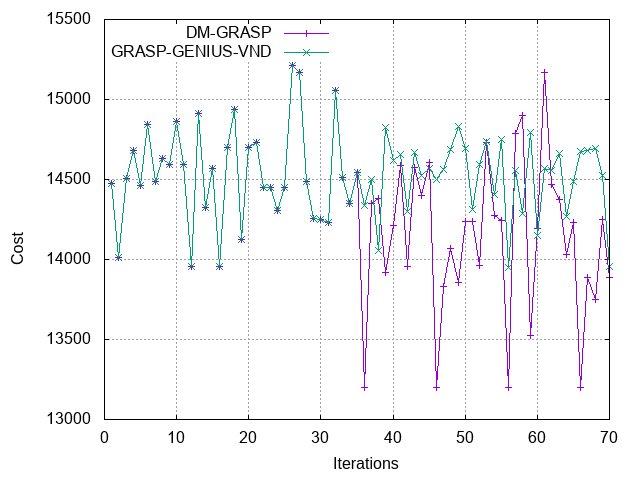
\includegraphics[width=0.8\textwidth]{construcao_grasp_dm-grasp.png}%
\caption{Construction phase of DM-GRASP}
\label{fig:cdm}
\end{figure}


\begin{figure}[!h]
	\centering
	
	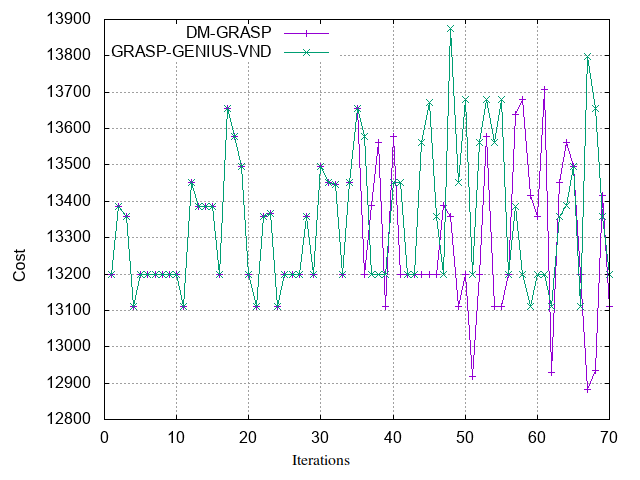
\includegraphics[width=0.8\textwidth]{buscalocal_grasp_dm-grasp.png}%
	\caption{Local search phase of DM-GRASP}
	\label{fig:bldm}
\end{figure}

The impact of using mined patterns with MDM-GRASP was also analysed, and Figures \ref{fig:cmdm} and \ref{fig:blmdm} show similar trends for the construction and local search phases of both data mining strategies. MDM-GRASP performed the data mining procedure four times during the experiment, after iterations 10, 34, 48, and 62. Unlike DM-GRASP, MDM-GRASP gradually reduces the cost of solutions obtained by construction as patterns are extracted more than once.

The proposed strategies also demonstrate a better exploration of the search space, which is often inefficient with state-of-the-art heuristics. For instance, in Figure \ref{fig:blmdm}, the value obtained by the GRASP-GENIUS-RVND local search remains unchanged during several iterations, but this behaviour is less likely to occur when MD is applied.



\begin{figure}[!h]
	\centering
	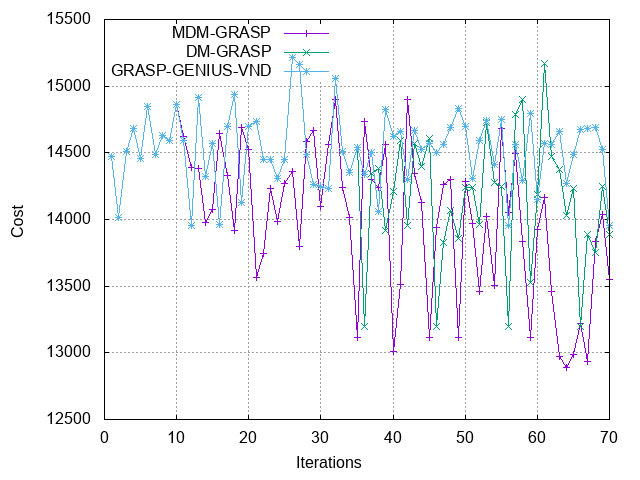
\includegraphics[width=0.7\textwidth]{construcao_mdm_dm_grasp.png}
	\caption{Construction phase of MDM-GRASP}
	\label{fig:cmdm}
\end{figure}


\begin{figure}[!h]
	\centering
	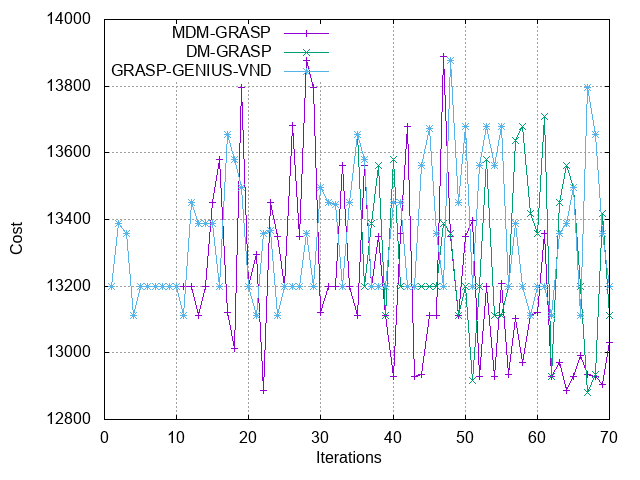
\includegraphics[width=0.7\textwidth]{buscalocal_mdm_dm_grasp.png}
	\caption{Local search phase of MDM-GRASP}
	\label{fig:blmdm}
\end{figure}

Tables \ref{tab:dm-grasp} and \ref{tab:mdm-grasp} demonstrated that the main benefit of applying MD in the state-of-the-art heuristic is reducing computational time. To illustrate this, Figures \ref{fig:md-tempo-c} and \ref{fig:md-tempo-bl} show the behaviour of the construction and local search phases in terms of computational time for GRASP-GENIUS-RVND, DM-GRASP, and MDM-GRASP, using instance g\_kroA150\_VT30\_T30\_W90\_50 with 70 iterations. The figures reveal that, for all strategies, the local search phase takes more time than the construction phase. In the DM-GRASP strategy, the MD process is executed after iteration 35. Figure \ref{fig:md-tempo-c} demonstrates that from this point on, the computational time spent on the construction phase is reduced. Originally, the construction of a route begins by randomly selecting three vertices, after which vertices are inserted into the route until all problem constraints are satisfied. With the application of MD, vertices are inserted using mined patterns, which typically contain more than three vertices, reducing the number of insertions needed to satisfy all the constraints and reducing the computational time spent.

The RVND heuristic is used for the GRASP-GENIUS-RVND local search, which explores all types of neighbourhoods until there are no more improvements. Each time a new improvement is made, RVND restarts its process from the first neighbourhood in the list. Since the solutions generated from pattern construction are typically closer to an optimal solution, as seen in Figure \ref{fig:md-tempo-bl}, exploring all neighbourhoods is completed faster as fewer improvements are made, and RVND returns fewer times to the first neighbourhood in the list.

In the MDM-GRASP strategy, the data mining process is performed multiple times. As shown in Figures \ref{fig:md-tempo-c} and \ref{fig:md-tempo-bl}, MDM-GRASP behaves similarly to DM-GRASP until the first mining process is performed. From this point on, as more mining processes are executed, the computational times for the construction and local search phases are gradually and slightly reduced.

\begin{figure}[!h]
	\centering
	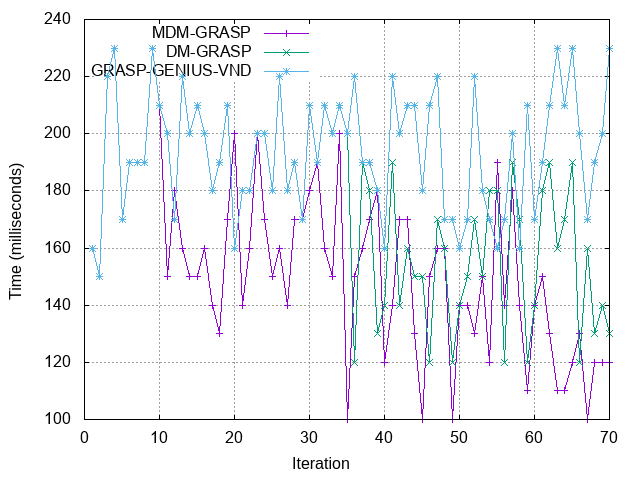
\includegraphics[width=0.7\textwidth]{md-tempo-construcao.png}
	\caption{Construction phase}
	\label{fig:md-tempo-c}
\end{figure}

\begin{figure}[!h]
	\centering
	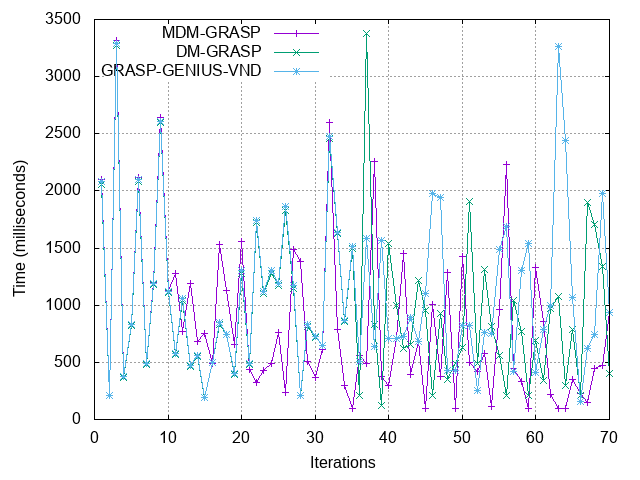
\includegraphics[width=0.7\textwidth]{md-tempo-bl.png}
	\caption{Local search phase}
	\label{fig:md-tempo-bl}
\end{figure}

\subsection{Statistical tests}

Statistical significance tests (SSTs) were conducted for all instances to enhance the assessment of the proposed methods. The purpose of this test is to determine, in statistical terms, whether the results obtained by the heuristics show a statistical difference, thus reinforcing the significance of applying MD or not.

Typically, this type of test is used to evaluate algorithms that involve random components and to determine whether the difference between their means is due to the superiority of one of the algorithms or simply to the randomness present in the methods. This study used the non-parametric statistical test of Friedman \cite{siegal1956nonparametric}, available in the R package \cite{r-package}. This test does not require the analyzed sample to follow a normal distribution.

To perform the test, the costs obtained from ten runs of each heuristic were considered, with a $p$-value of 0.05 and two hypotheses:

\begin{itemize}
\item Null hypothesis ($H_0$): There is no difference between the means obtained by the two methods; and
\item Alternative hypothesis ($H_1$): There is a difference between the means obtained by the two methods.
\end{itemize}


In this sense, $H_0$ will be rejected with 95\% certainty if, for each instance, the test of \textit{Friedman} \cite{siegal1956nonparametric} returns a value less than the defined $p$-value.
If $H_0$ is rejected, the alternative hypothesis $H_1$ is considered.

In Table \ref{tab:sig1}, for each pair of compared heuristics, the number of wins, losses and ties in terms of the best solution, average solution and average time spent is shown. For the solution mean, the values in parentheses indicate the number of statistically significant results. MDM-GRASP was not directly compared with the state-of-the-art heuristic, but with DM-GRASP in Table \ref{tab:mdm-grasp}. Table \ref{tab:sig1}, presents a summary of what can be deduced from Tables \ref{tab:dm-grasp} and \ref{tab:mdm-grasp}, about a comparison between MDM- GRASP and GRASP-GENIUS-RVND.

\begin{table}[!h]
\centering
\caption{Summary of results and statistical significance test between GRASP-GENIUS-RVND and MDM-GRASP.}
\label{tab:sig1}
\begin{tabular}{llll}
\hline
& Best Sol. & Average Sol. & Average T(s) \\
\hline
\begin{tabular}[c]{@{}l@{}}Win\\ MDM-GRASP\end{tabular} & 13 & 41 (10)& 105 \\ \hline
Ties & 90 & 50 & 0 \\ \hline
\begin{tabular}[c]{@{}l@{}}Win\\ GRASP-GENIUS-RVND\end{tabular} & 4 & 16 (0) & 2\\
\hline
\end{tabular}
\end{table}

Regarding the best solution, MDM-GRASP was superior in 13, tied in 90, and lost in 4 instances. Regarding the average solution, the mining heuristic won in 41 cases, ten statistically significant cases, tied in 50, and lost in 16 instances. This statistical test showed that the significant results obtained are concentrated in the larger instances, including gr202\_R39\_T122\_W41\_25, gr229\_R45\_T46\_W138\_25, lin318\_R108\_T105\_W105 \_50, rd400\_R80\_T240\_W80\_25, among others. As already noted in previous sections, the application of data mining reduces the computational time of the heuristics. With MDM-GRASP, it was no different, being faster than the state-of-the-art heuristic in 105 of the 107 instances tested and with an average CPU-time reduction of 23.55\% per instance.

\subsection{TTTPlots}

A final comparison was made between the proposed methods and the state-of-the-art, using \textit{Time-to-target plots} (\texttt{TTTplots}) \cite{aiex2007ttt}. These types of plots are used to analyse the behaviour of algorithms with random components and show the cumulative probability of an algorithm to find a solution better than or equal to a predefined target solution value in a specific running time.

The TTTplots illustrated in Figure \ref{fig:tttplots1} were generated from 100 executions of the GRASP-GENIUS-RVND and MDM-GRASP methods using the instance g\_kroA150\_VT30\_T30\_W90\_50, and  seeds ranging from 1 to 100. For the behaviour analysis, a difficult target value was chosen, the value of the best solution reported by GRASP-GENIUS-RVND (12918).

\begin{figure}[!h]
\centering
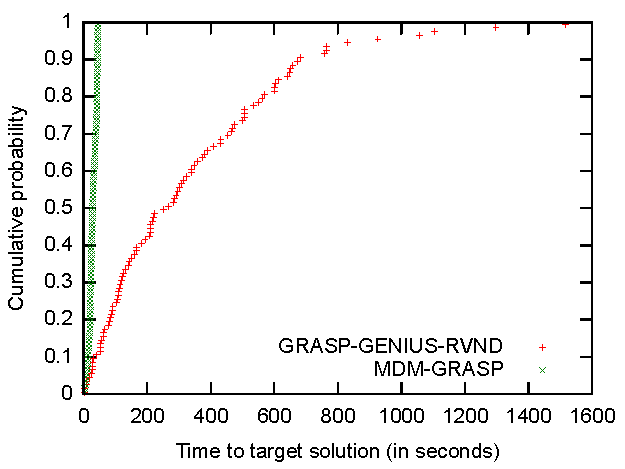
\includegraphics[width=0.7\textwidth]{tttplot.pdf}
\caption{TTTplots for instance g\_kroA150\_VT30\_T30\_W90\_50, target: 12962.}
\label{fig:tttplots1}%
\end{figure}

From Figure \ref{fig:tttplots1}, a significant difference can be seen between the curves of the compared heuristics. After 561 seconds of execution, GRASP-GENIUS-RVND reaches the target with a probability of 79\%, while with that same chance, MDM-GRASP only needs 41.71 seconds to reach the target.

\section{Conclusions}

\label{sec:conclusions}

In conclusion, this study proposed two hybrid heuristics, DM-GRASP and MDM-GRASP, which utilize data mining techniques over a state-of-the-art heuristic, GRASP-GENIUS-RVND. The heuristics were evaluated using various methods, including the re-execution of all experiments and the use of statistical significance tests. The results showed that both DM strategies outperformed the state-of-the-art heuristic regarding solution quality and CPU time.

Furthermore, the heuristics were able to significantly reduce the execution time, which confirms the effectiveness of using data mining techniques. MDM-GRASP was the best-performing heuristic among the three compared, achieving an 88.1\% reduction in execution time for a specific instance.

Despite the promising results, this study also has some limitations. First, the proposed approach may not apply to all combinatorial optimization problems since different solution structures may require different techniques to mine the patterns. Secondly, the effectiveness of the approach can be affected by the quality and quantity of the available data, a reduced number of iterations in the base heuristic, for example, can compromise the quality of the data. Finally, the proposed approach assumes that patterns in high-quality solutions will lead to better solutions; therefore, the base heuristic itself must be of good quality.

Future work will focus on combining MDM-GRASP with integer programming techniques to explore the possibility of using mined patterns to assist in the exact resolution of integer programming models through warm starts or guiding variable selection for branching. Overall, this study has demonstrated the potential of using data mining techniques to enhance the performance of existing heuristics.

%\bibliographystyle{model1-num-names}
\bibliographystyle{apalike}

% Loading bibliography database
\bibliography{cas-refs}


\end{document}

